\documentclass[aspectratio=169]{beamer}

% Fonts
\usepackage{lmodern}
\usepackage[english]{babel}

% Math and symbols
\usepackage{amsmath}
\usepackage{amsfonts}
\usepackage{amssymb}

% Graphics and figures
\usepackage{graphicx}
\usepackage{fontawesome5}
\usepackage{worldflags}
\usepackage{qrcode}

% TikZ for diagrams
\usepackage{tikz}
\usetikzlibrary{positioning,shapes,arrows,decorations.pathreplacing,decorations.pathmorphing}

% Tables
\usepackage{booktabs}
\usepackage{array}

% Citations and references
\usepackage[backend=biber,style=authoryear,dashed=false,url=true,doi=false,eprint=false,maxnames=99,maxcitenames=1]{biblatex}

% Appendix frame numbering
\usepackage{appendixnumberbeamer}

% Beamer theme
\usetheme{moloch}

% Clean navigation: just frame numbers
\setbeamertemplate{navigation symbols}{}

% Bibliography customizations
\AtEveryBibitem{%
  \clearfield{note}%
  \clearfield{pagetotal}%
  \clearfield{pages}%
  \clearfield{isbn}%
  \clearfield{issn}%
  \clearfield{archivePrefix}%
  \clearfield{eprint}%
  \clearfield{primaryClass}%
  \clearname{editor}%
  \clearfield{urldate}%
  \clearfield{urlyear}%
  \clearfield{urlmonth}%
  \clearfield{urlday}%
}

% Custom citation format: [FirstAuthor Year]
\DeclareFieldFormat{citehyperref}{%
  \DeclareFieldAlias{bibhyperref}{noformat}%
  \bibhyperref{#1}}

\DeclareCiteCommand{\cite}[\mkbibparens]
  {\usebibmacro{prenote}}
  {\usebibmacro{citeindex}%
   \printtext[citehyperref]{\usebibmacro{cite}}}
  {\multicitedelim}
  {\usebibmacro{postnote}}

\renewcommand{\mkbibparens}[1]{\mkbibbrackets{#1}}

% Smaller bibliography font for slides
\renewcommand*{\bibfont}{\footnotesize}

\renewbibmacro{in:}{}

% Titles link to the paper instead of printing the URL
\DeclareFieldFormat[article,inproceedings,misc,online,report,unpublished,book,incollection,thesis]{title}{%
  \iffieldundef{url}{\mkbibemph{#1}}{\href{\thefield{url}}{\mkbibemph{#1}}}}

% Clean source citation: "Paper Title" [Author Year]
% Shows at bottom of slide, clickable to bibliography
\DeclareCiteCommand{\sourcecite}{}
  {\textit{\printfield{title}}%
   \hspace{0.4em}%
   \printtext[citehyperref]{\mkbibbrackets{\printnames{labelname}\addcomma\addspace\printfield{year}}}%
  }{\newline}{}

\newcommand{\source}[1]{%
  \vfill
  {\raggedright\scriptsize\color{gray}\sourcecite{#1}\par}%
}

\newcommand{\coursetitle}{Are we expecting RSI within the next 2 years?}
\newcommand{\instructor}{Julian Schulz}
\newcommand{\institution}{}

% \paperfig{image.png}{caption.txt}
% Shows a centered image with caption text read from file below it.
% If the caption file does not exist, no caption is shown.
\usepackage{catchfile}

\newcommand{\paperfig}[2]{%
  \begin{center}
  \includegraphics[width=0.85\textwidth,height=0.6\textheight,keepaspectratio]{#1}%
  \end{center}%
  \ifx\relax#2\relax\else
    \IfFileExists{#2}{%
      \CatchFileDef{\captiontext}{#2}{\endlinechar=-1}%
      {\tiny\captiontext}%
    }{}%
  \fi
}

\addbibresource{bib/refs.bib}
\addbibresource{bib/manual.bib}

\graphicspath{
  {content/01_intro/figures/}
  {content/02_what_rsi_looks_like/figures/}
  {content/03_consequences/figures/}
  {content/04_evidence/figures/}
  {content/05_counterarguments/figures/}
  {content/06_implications/figures/}
}

\title{Recursive Self-Improvement}
\author{\instructor}
\institute{\scriptsize\color{gray}Principles of Intelligence (PIRAMID) \,·\, Meridian Visiting Researcher Programme}
\date{}

\begin{document}

\begin{frame}
\titlepage
\begin{tikzpicture}[remember picture, overlay]
\node[anchor=south east, align=center, inner sep=0] at ([xshift=-0.8cm, yshift=0.8cm]current page.south east) {\qrcode[height=2.2cm]{https://github.com/wusche1/RSI_talk/raw/main/output/main.pdf}\\[0.3em]{\scriptsize Slides}};
\end{tikzpicture}
\end{frame}

\begin{frame}{}
\vspace{1em}
\begin{columns}[c]
\column{0.68\textwidth}
``I think we're looking at something like maybe a 1/3 chance that we have superintelligence within one year on the current development trajectory, if we do not slow.''

\vspace{1.2em}
``I would say we are looking more like a 10\% risk [of AI takeover] than a 1\% risk over the next year.''
\column{0.27\textwidth}
\centering
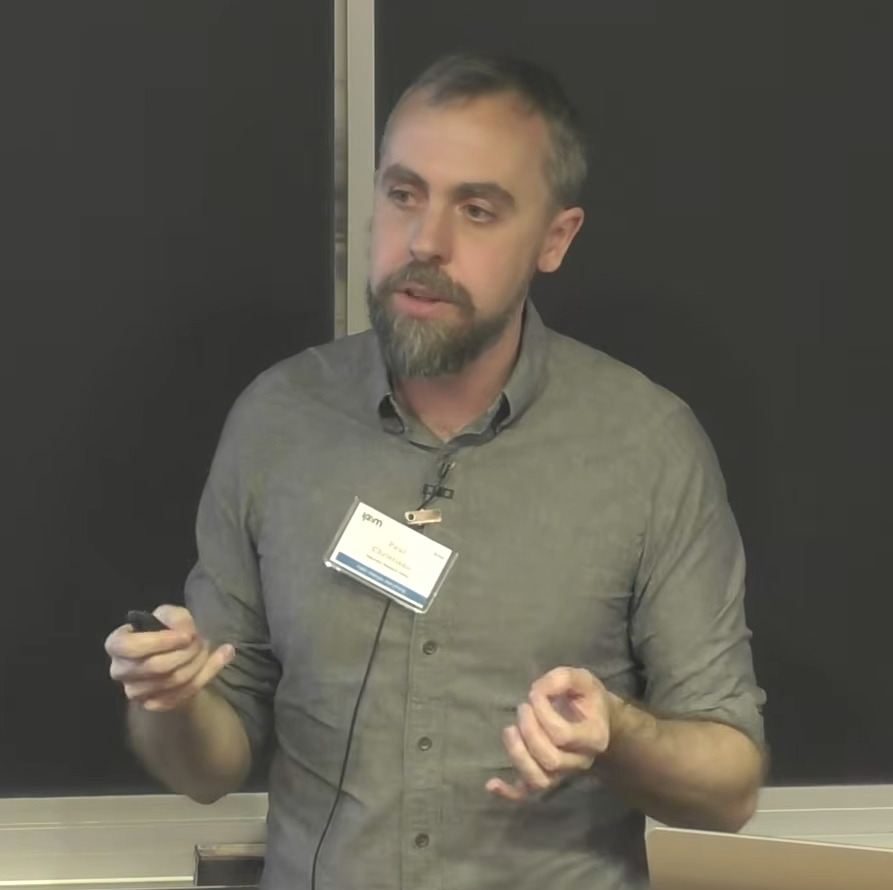
\includegraphics[width=0.75\linewidth]{christiano}

\vspace{0.4em}
\textbf{Paul Christiano}

\vspace{0.2em}
{\footnotesize OpenAI board member\\
Former head of the US AI Safety Institute\\
Inventor of RLHF}

{\tiny\color{gray}Photo: IPAM at UCLA, CC BY 4.0}
\end{columns}

\source{patel2026a}
\end{frame}

\begin{frame}{}
\centering
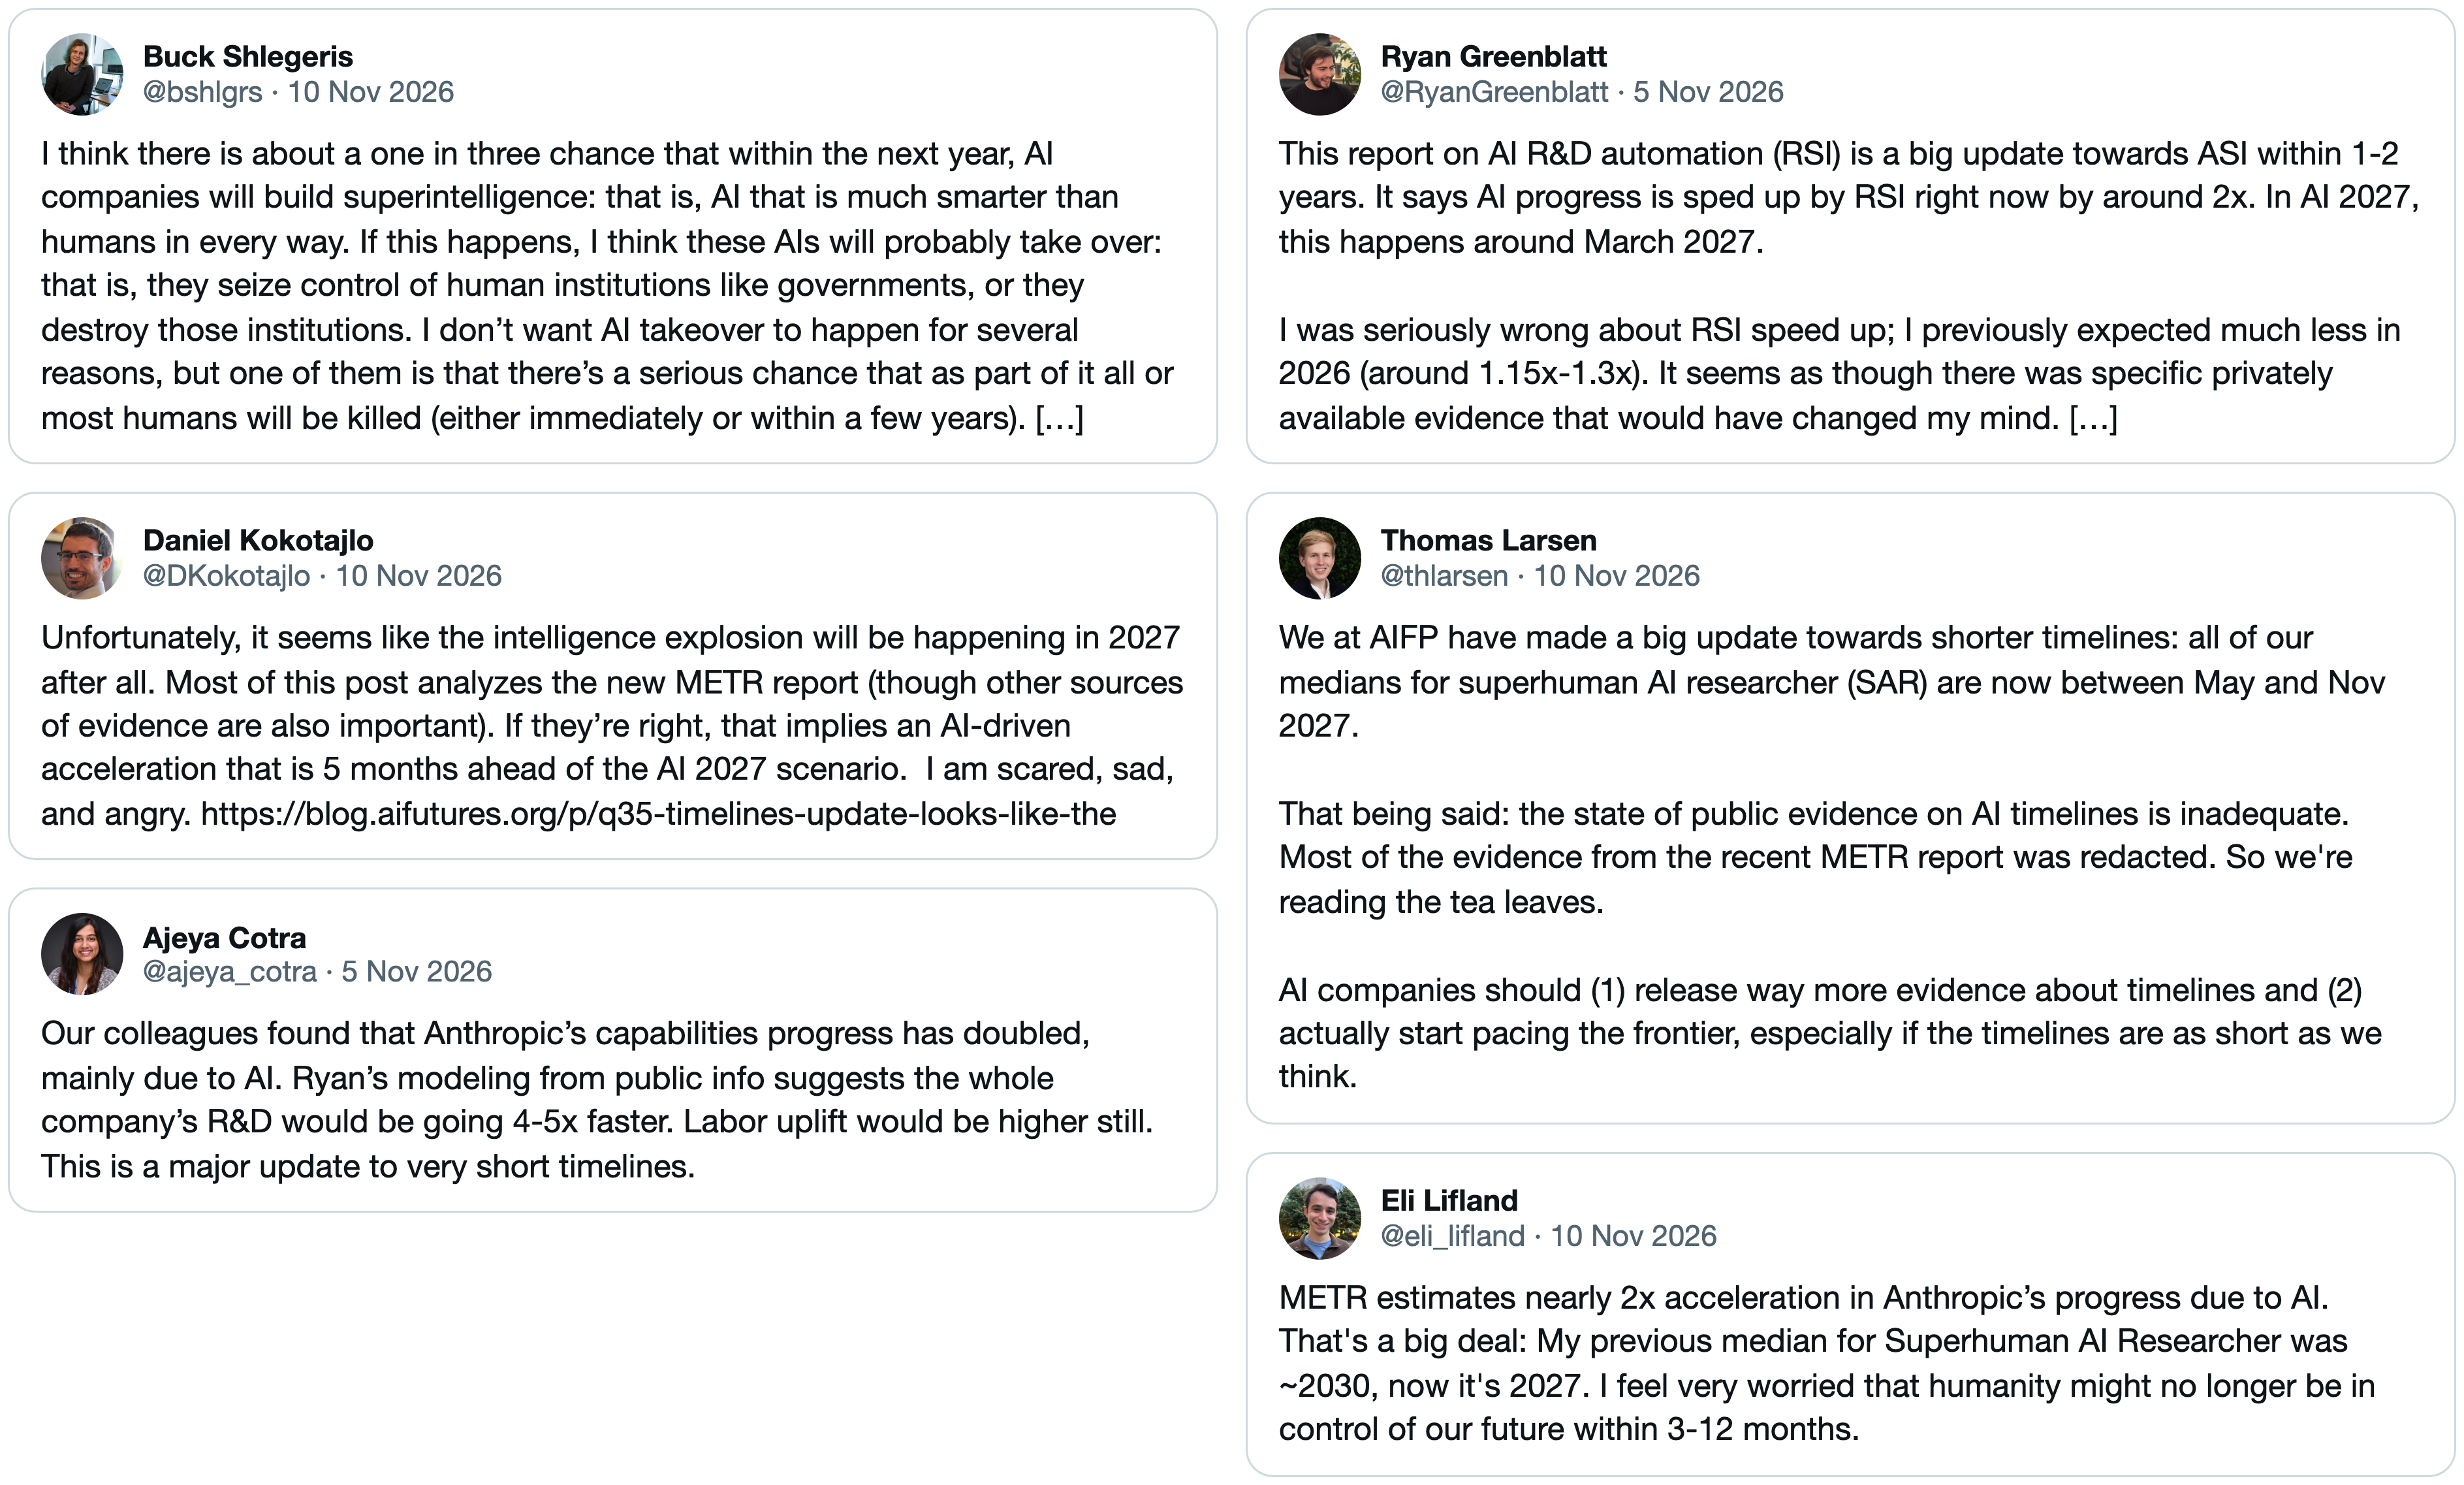
\includegraphics[width=\textwidth,height=0.86\textheight,keepaspectratio]{tweets/collage}

\vfill
{\scriptsize\color{gray}Posts on X, 5--10 November 2026:
\href{https://x.com/bshlgrs/status/2120271165692461316}{Shlegeris},
\href{https://x.com/DKokotajlo/status/2120204075803500595}{Kokotajlo},
\href{https://x.com/ajeya_cotra/status/2118448038356390177}{Cotra},
\href{https://x.com/thlarsen/status/2120207830787719410}{Larsen},
\href{https://x.com/RyanGreenblatt/status/2118447235289817503}{Greenblatt},
\href{https://x.com/eli_lifland/status/2120238246089437403}{Lifland}}
\end{frame}

\begin{frame}{}
\centering
\vfill
{\LARGE ``Extraordinary claims require\\[0.3em] extraordinary evidence.''}

\vspace{1.5em}
Carl Sagan, \textit{Cosmos} (1980)
\vfill
\end{frame}

\begin{frame}{Overview}
\begin{enumerate}
\item What is RSI?
\item Consequences of RSI
\item Evidence for RSI
\item Arguments against RSI
\item What do we do now?
\end{enumerate}
\end{frame}


\section{What Is RSI?}
\begin{frame}{Recursive Self-Improvement}
\begin{center}
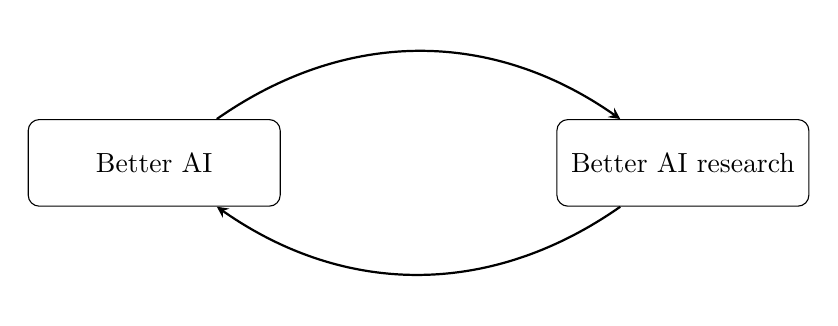
\begin{tikzpicture}[every node/.style={draw, rounded corners, align=center, minimum height=1.1cm, minimum width=3.2cm}, >=stealth]
\node (a) {Better AI};
\node (b) [right=3.5cm of a] {Better AI research};
\draw[->, thick, bend left=35] (a) to (b);
\draw[->, thick, bend left=35] (b) to (a);
\end{tikzpicture}
\end{center}
\vspace{1em}
\begin{itemize}
\item AIs are becoming human-level at more and more tasks
\item At some point, one of those tasks is AI research itself
\end{itemize}
\end{frame}

\begin{frame}{What Goes Into a Frontier Model?}
\centering
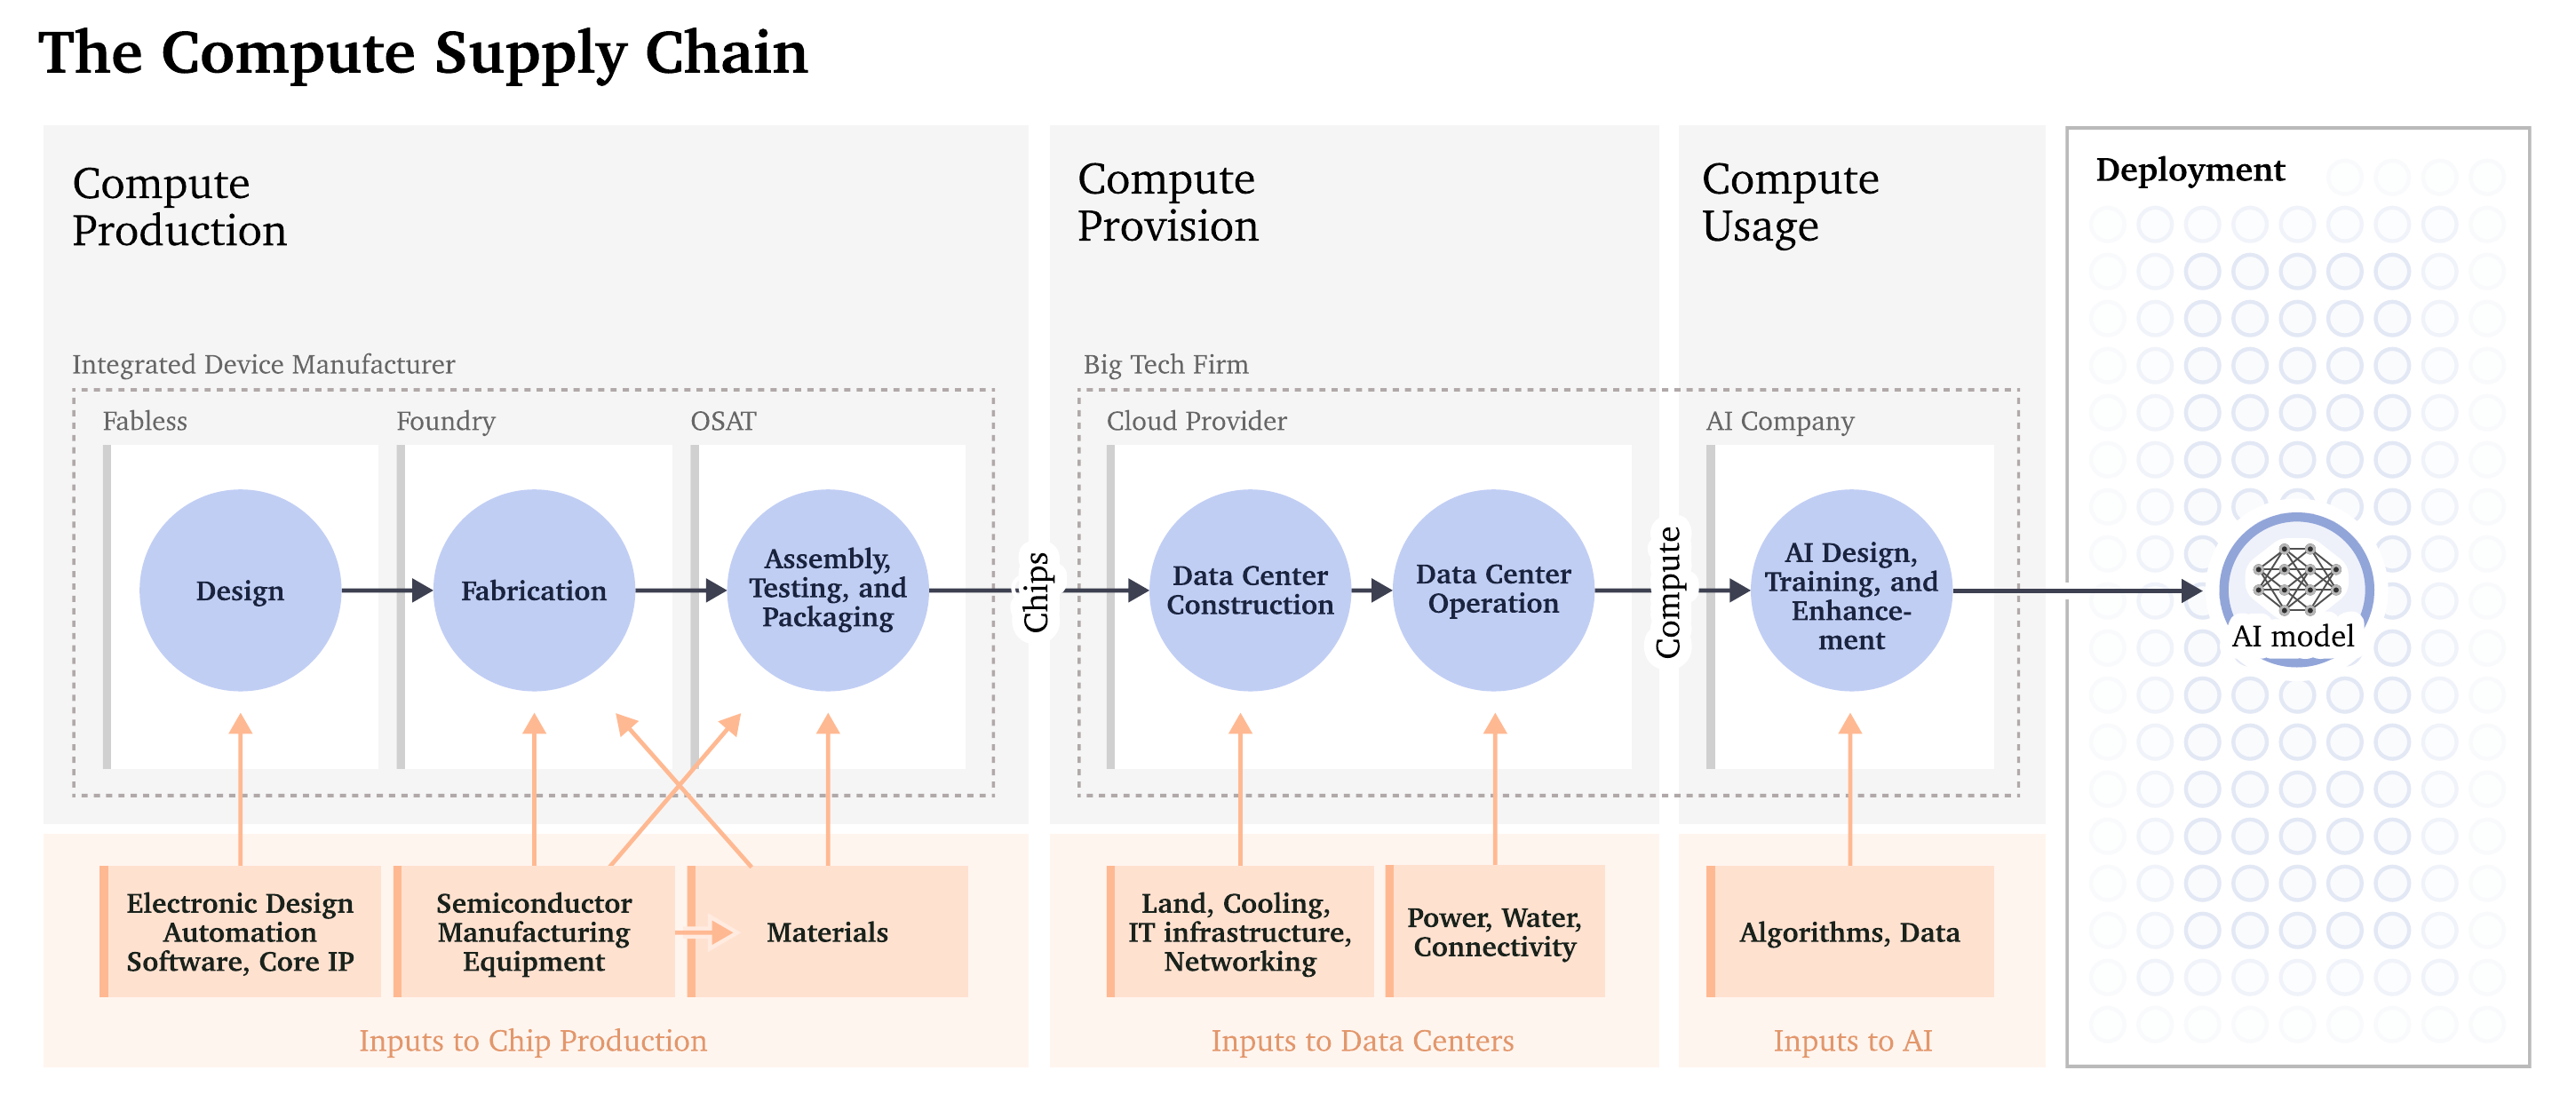
\includegraphics[width=\textwidth]{sastry2024_fig10_compute_supply_chain}
\source{sastry2024}
\end{frame}

\begin{frame}{Compute Is Growing Exponentially}
\begin{columns}[c]
\column{0.5\textwidth}
\centering
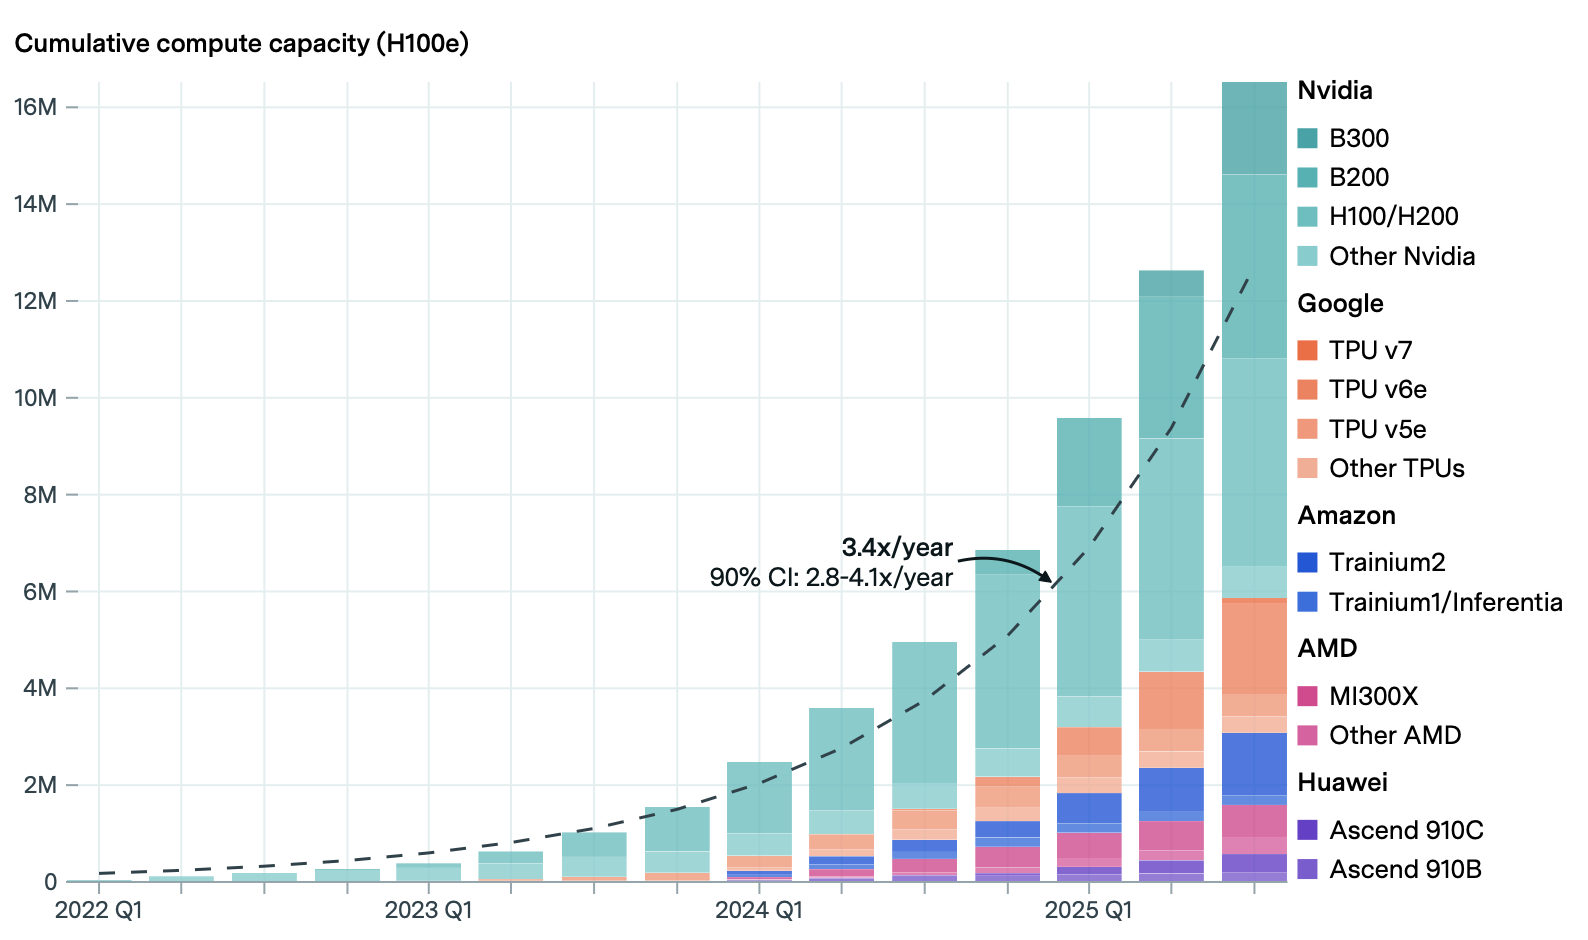
\includegraphics[width=\linewidth]{epoch_chip_stock}

{\small All AI chips in the world: \textbf{3.4$\times$ per year}}
\column{0.5\textwidth}
\centering
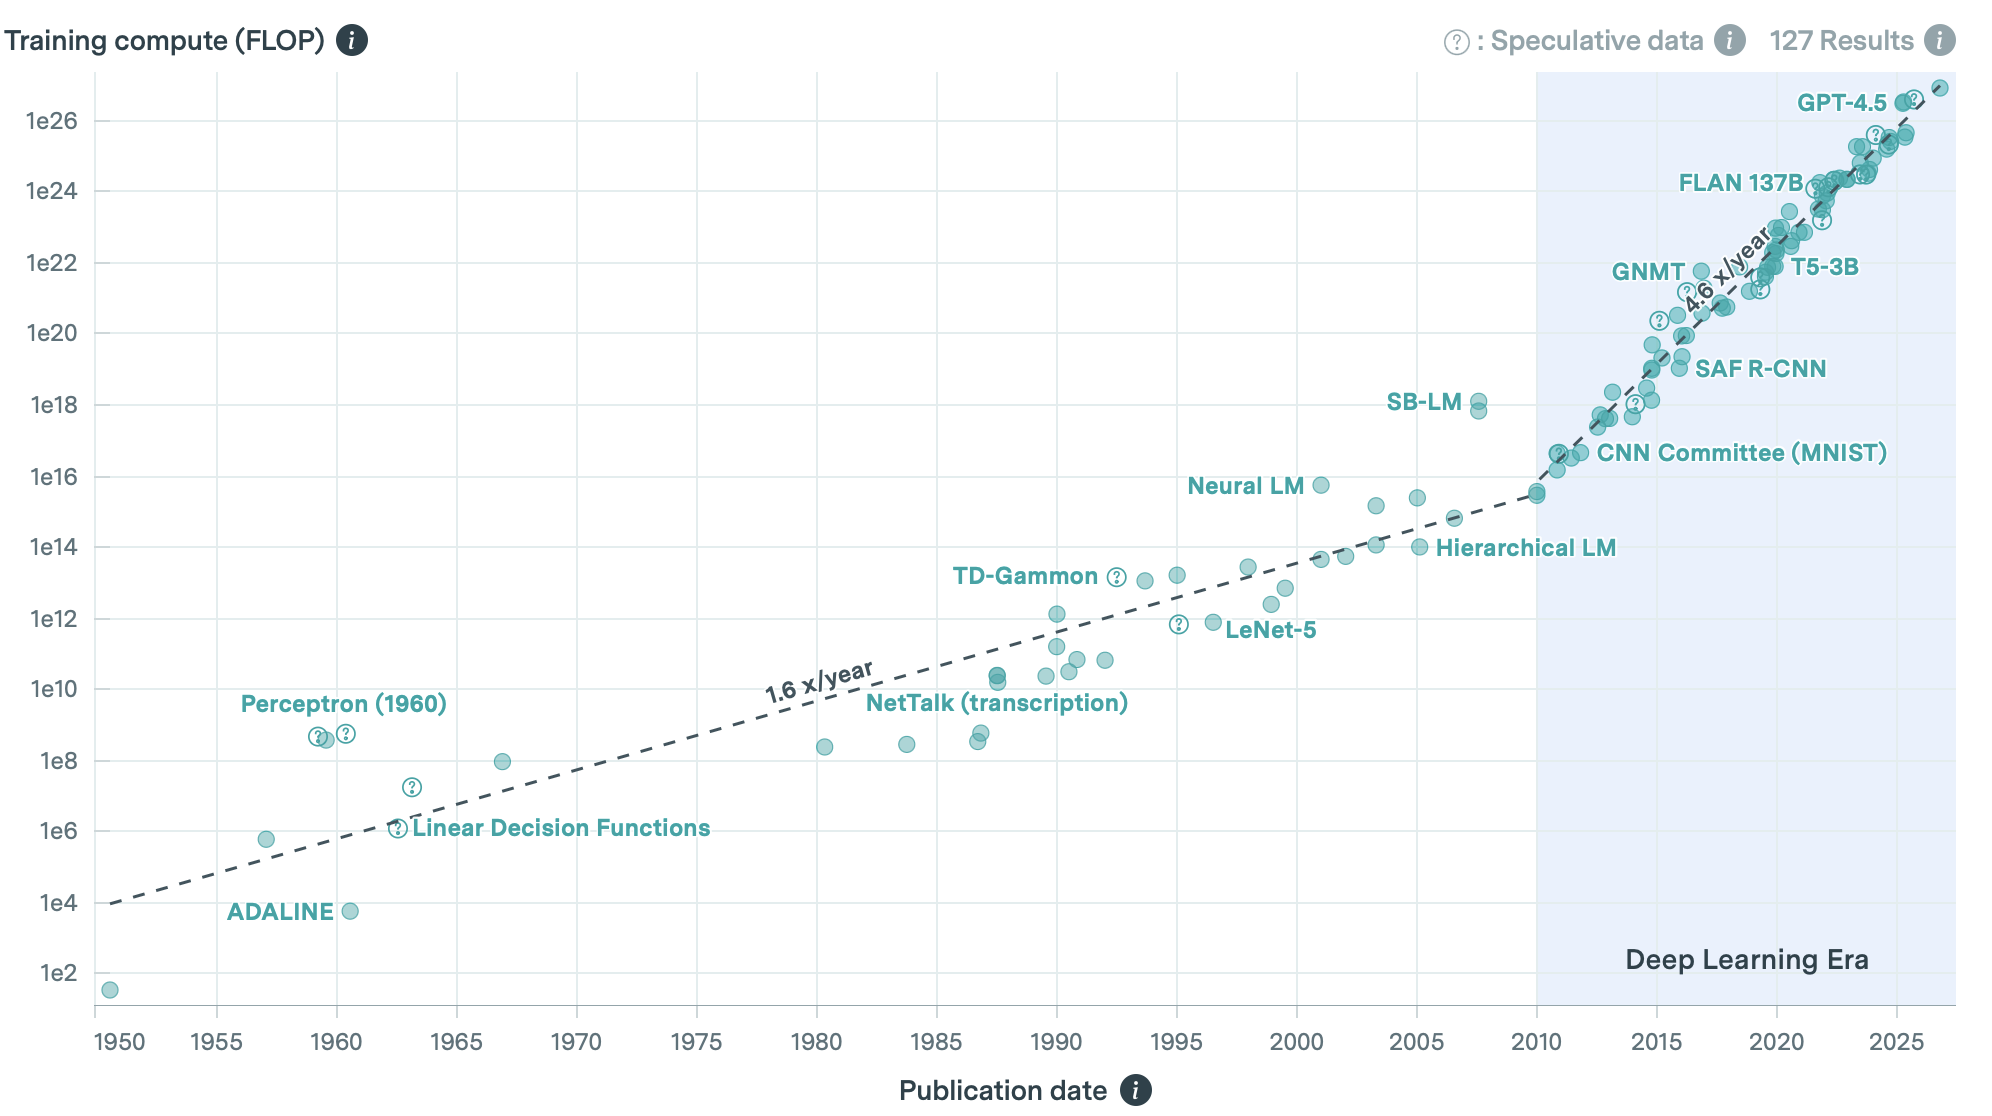
\includegraphics[width=\linewidth]{epoch_training_compute}

{\small Largest training runs: \textbf{4.6$\times$ per year}}
\end{columns}
\source{epochtrends2026,epochmodels2026}
\end{frame}

\begin{frame}{Algorithms Are Improving Exponentially}
\begin{columns}[c]
\column{0.42\textwidth}
\centering
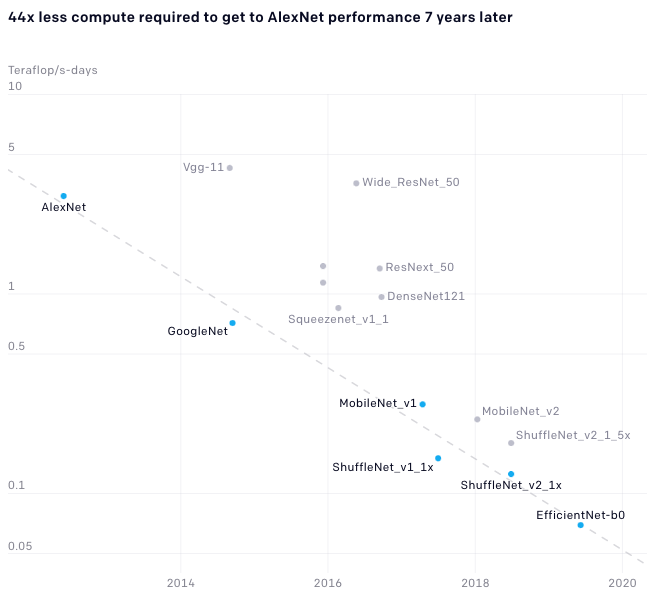
\includegraphics[width=\linewidth]{hernandez_alexnet_efficiency}

{\small Image recognition, 2012--2019:\\ \textbf{44$\times$ less compute}}
\column{0.56\textwidth}
\centering
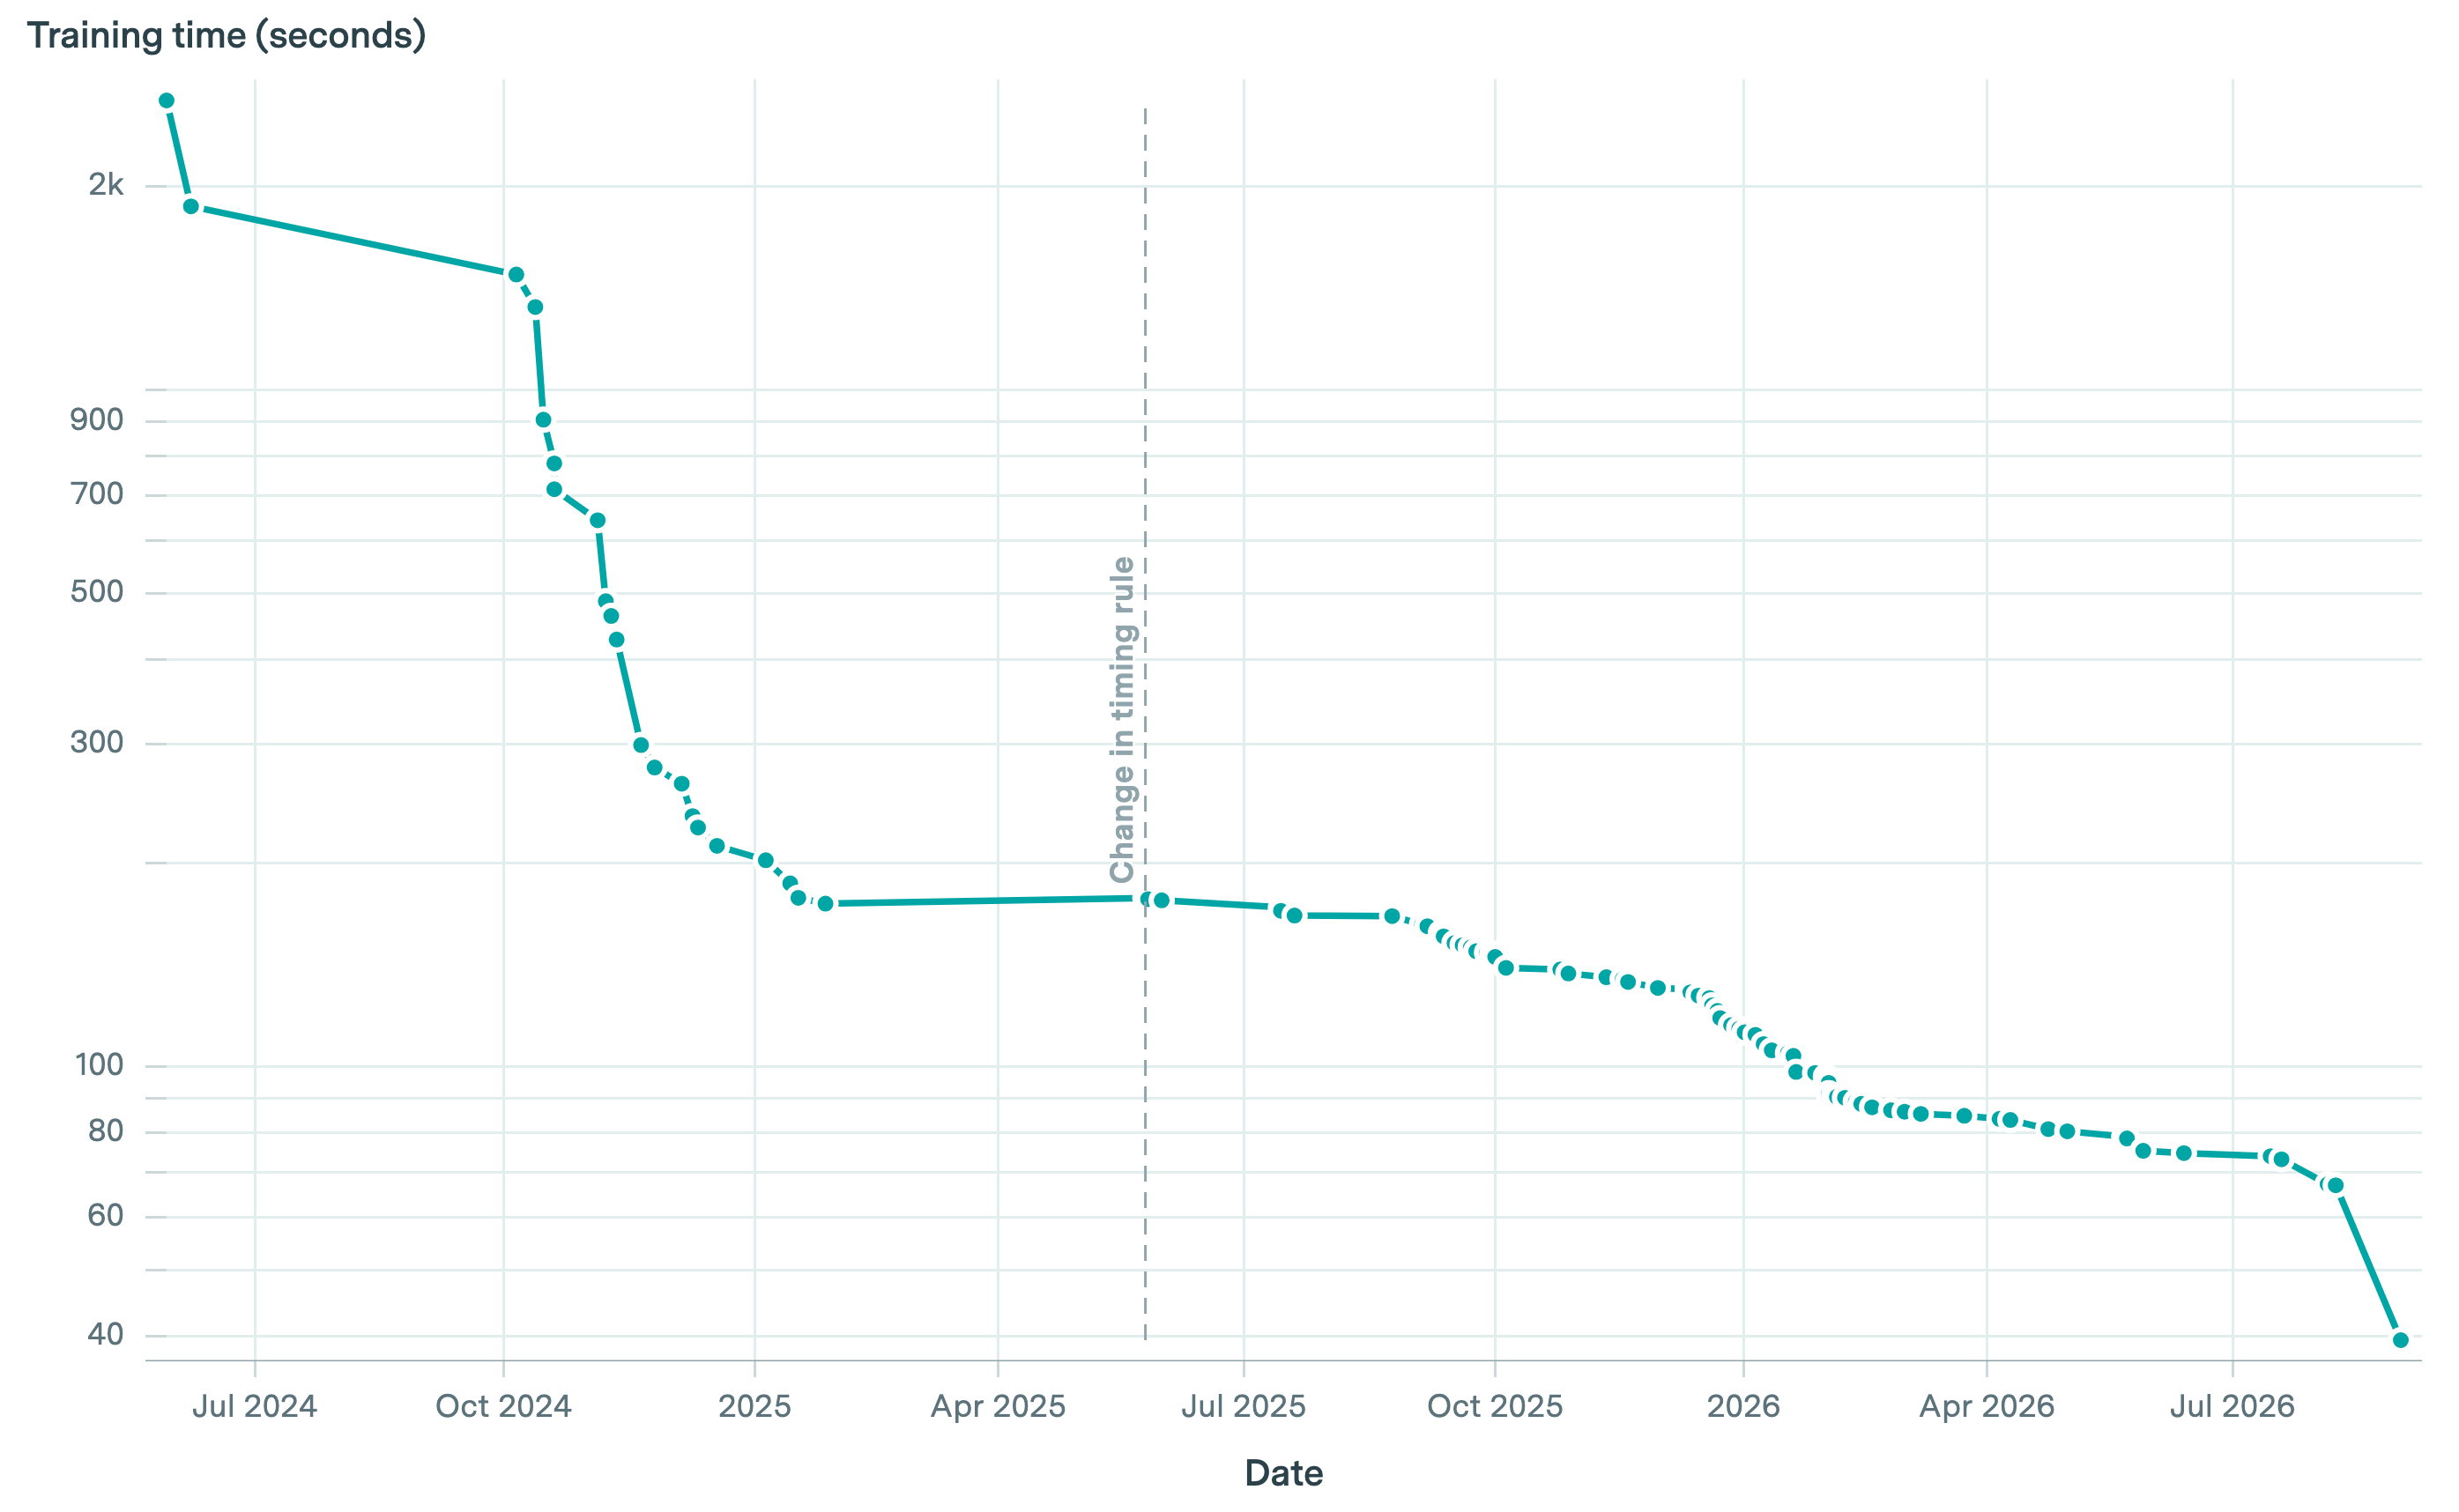
\includegraphics[width=\linewidth]{epoch_nanogpt_speedrun}

{\small Same model, same hardware, same data, 2024--2026:\\ \textbf{45 minutes $\to$ 40 seconds}}
\end{columns}
\source{hernandez2020,ai2026}
\end{frame}

\begin{frame}{Not All Inputs Depend on AI in the Same Way}
\begin{columns}[c]
\column{0.5\textwidth}
\centering
\textbf{Weak recursion}

\vspace{0.6em}
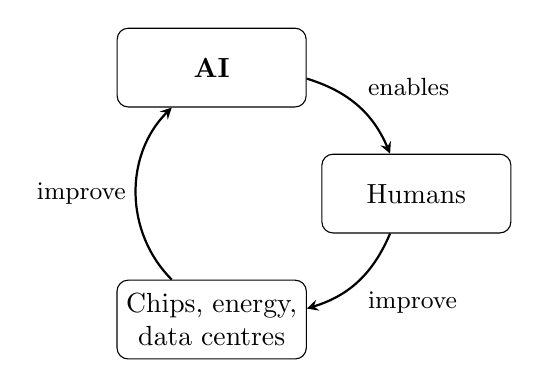
\begin{tikzpicture}[box/.style={draw, rounded corners, align=center, minimum height=1cm, minimum width=2.4cm}, >=stealth]
\node[box] (ai) at (0,3.2) {\textbf{AI}};
\node[box] (h) at (2.6,1.6) {Humans};
\node[box] (hw) at (0,0) {Chips, energy,\\data centres};
\draw[->, thick] (ai) to[bend left=25] node[above right] {\small enables} (h);
\draw[->, thick] (h) to[bend left=25] node[below right] {\small improve} (hw);
\draw[->, thick] (hw) to[bend left=45] node[left] {\small improve} (ai);
\end{tikzpicture}

\vspace{0.8em}
Through the human economy: \textbf{slow}
\column{0.5\textwidth}
\centering
\textbf{Strong recursion}

\vspace{0.6em}
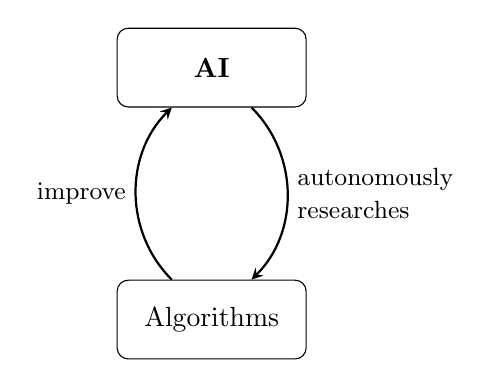
\begin{tikzpicture}[box/.style={draw, rounded corners, align=center, minimum height=1cm, minimum width=2.4cm}, >=stealth]
\node[box] (ai) at (0,3.2) {\textbf{AI}};
\node[box] (alg) at (0,0) {Algorithms};
\draw[->, thick] (ai) to[bend left=45] node[right, align=left] {\small autonomously\\\small researches} (alg);
\draw[->, thick] (alg) to[bend left=45] node[left] {\small improve} (ai);
\end{tikzpicture}

\vspace{0.8em}
Inside the data centre: \textbf{fast}
\end{columns}
\source{ball2026}
\end{frame}

\begin{frame}{Can an AI Build a Smarter AI?}
\begin{center}
\begin{tikzpicture}[scale=0.88, >=stealth]
\useasboundingbox (-1.5,-0.3) rectangle (11.5,7.7);
\draw[->] (0.4,0.4) -- (7.6,0.4) node[below left] {\small Intelligence of the AI doing the research};
\draw[->] (0.4,0.4) -- (0.4,7.3) node[above right, xshift=-0.3cm] {\small Smartest AI it can build};
\draw[gray, dashed] (0.4,0.4) -- (7,7) node[right, text=gray] {\small as smart as itself};
\only<1-5>{\draw[very thick, domain=1.3:4.3, samples=50] plot (\x, {\x + 0.5*(\x-2)*(4-\x)});}
\only<2>{
  \draw[thick, red!70!black, ->] (1.60,1.60) -- (1.60,1.12) -- (1.12,1.12);
  \node[red!70!black, align=left, anchor=west] at (2.6,1.2) {\small A weaker AI builds\\\small a weaker successor};
}
\only<3-5>{
  \draw[thick, green!50!black] (2.40,2.40) -- (2.40,2.72) -- (2.72,2.72);
  \node[green!50!black, align=left, anchor=west] at (4.6,2.6) {\small A stronger AI builds\\\small a stronger successor};
}
\only<4-5>{\draw[thick, green!50!black] (2.72,2.72) -- (2.72,3.18) -- (3.18,3.18);}
\only<5>{
  \draw[thick, green!50!black, ->] (3.18,3.18) -- (3.18,3.66) -- (3.66,3.66) -- (3.66,3.94) -- (3.94,3.94) -- (3.94,4.00) -- (4.00,4.00);
  \node[anchor=west] at (4.2,3.9) {\small the loop runs out of steam};
}
\only<6>{
  \draw[gray, domain=1.3:4.3, samples=50] plot (\x, {\x + 0.5*(\x-2)*(4-\x)});
  \draw[very thick, domain=1.3:6.9, samples=50] plot (\x, {\x + 0.222*(\x-2)*(6.5-\x)});
  \draw[thick, green!50!black, ->] (2.40,2.40) -- (2.40,2.76) -- (2.76,2.76) -- (2.76,3.40) -- (3.40,3.40) -- (3.40,4.36) -- (4.36,4.36) -- (4.36,5.48) -- (5.48,5.48) -- (5.48,6.27) -- (6.27,6.27) -- (6.27,6.49) -- (6.49,6.49) -- (6.49,6.50) -- (6.50,6.50);
  \node[anchor=north west] at (6.5,6.4) {\small limit of current hardware};
}
\end{tikzpicture}
\end{center}
\end{frame}

\begin{frame}{How Could This Play Out?}
\centering
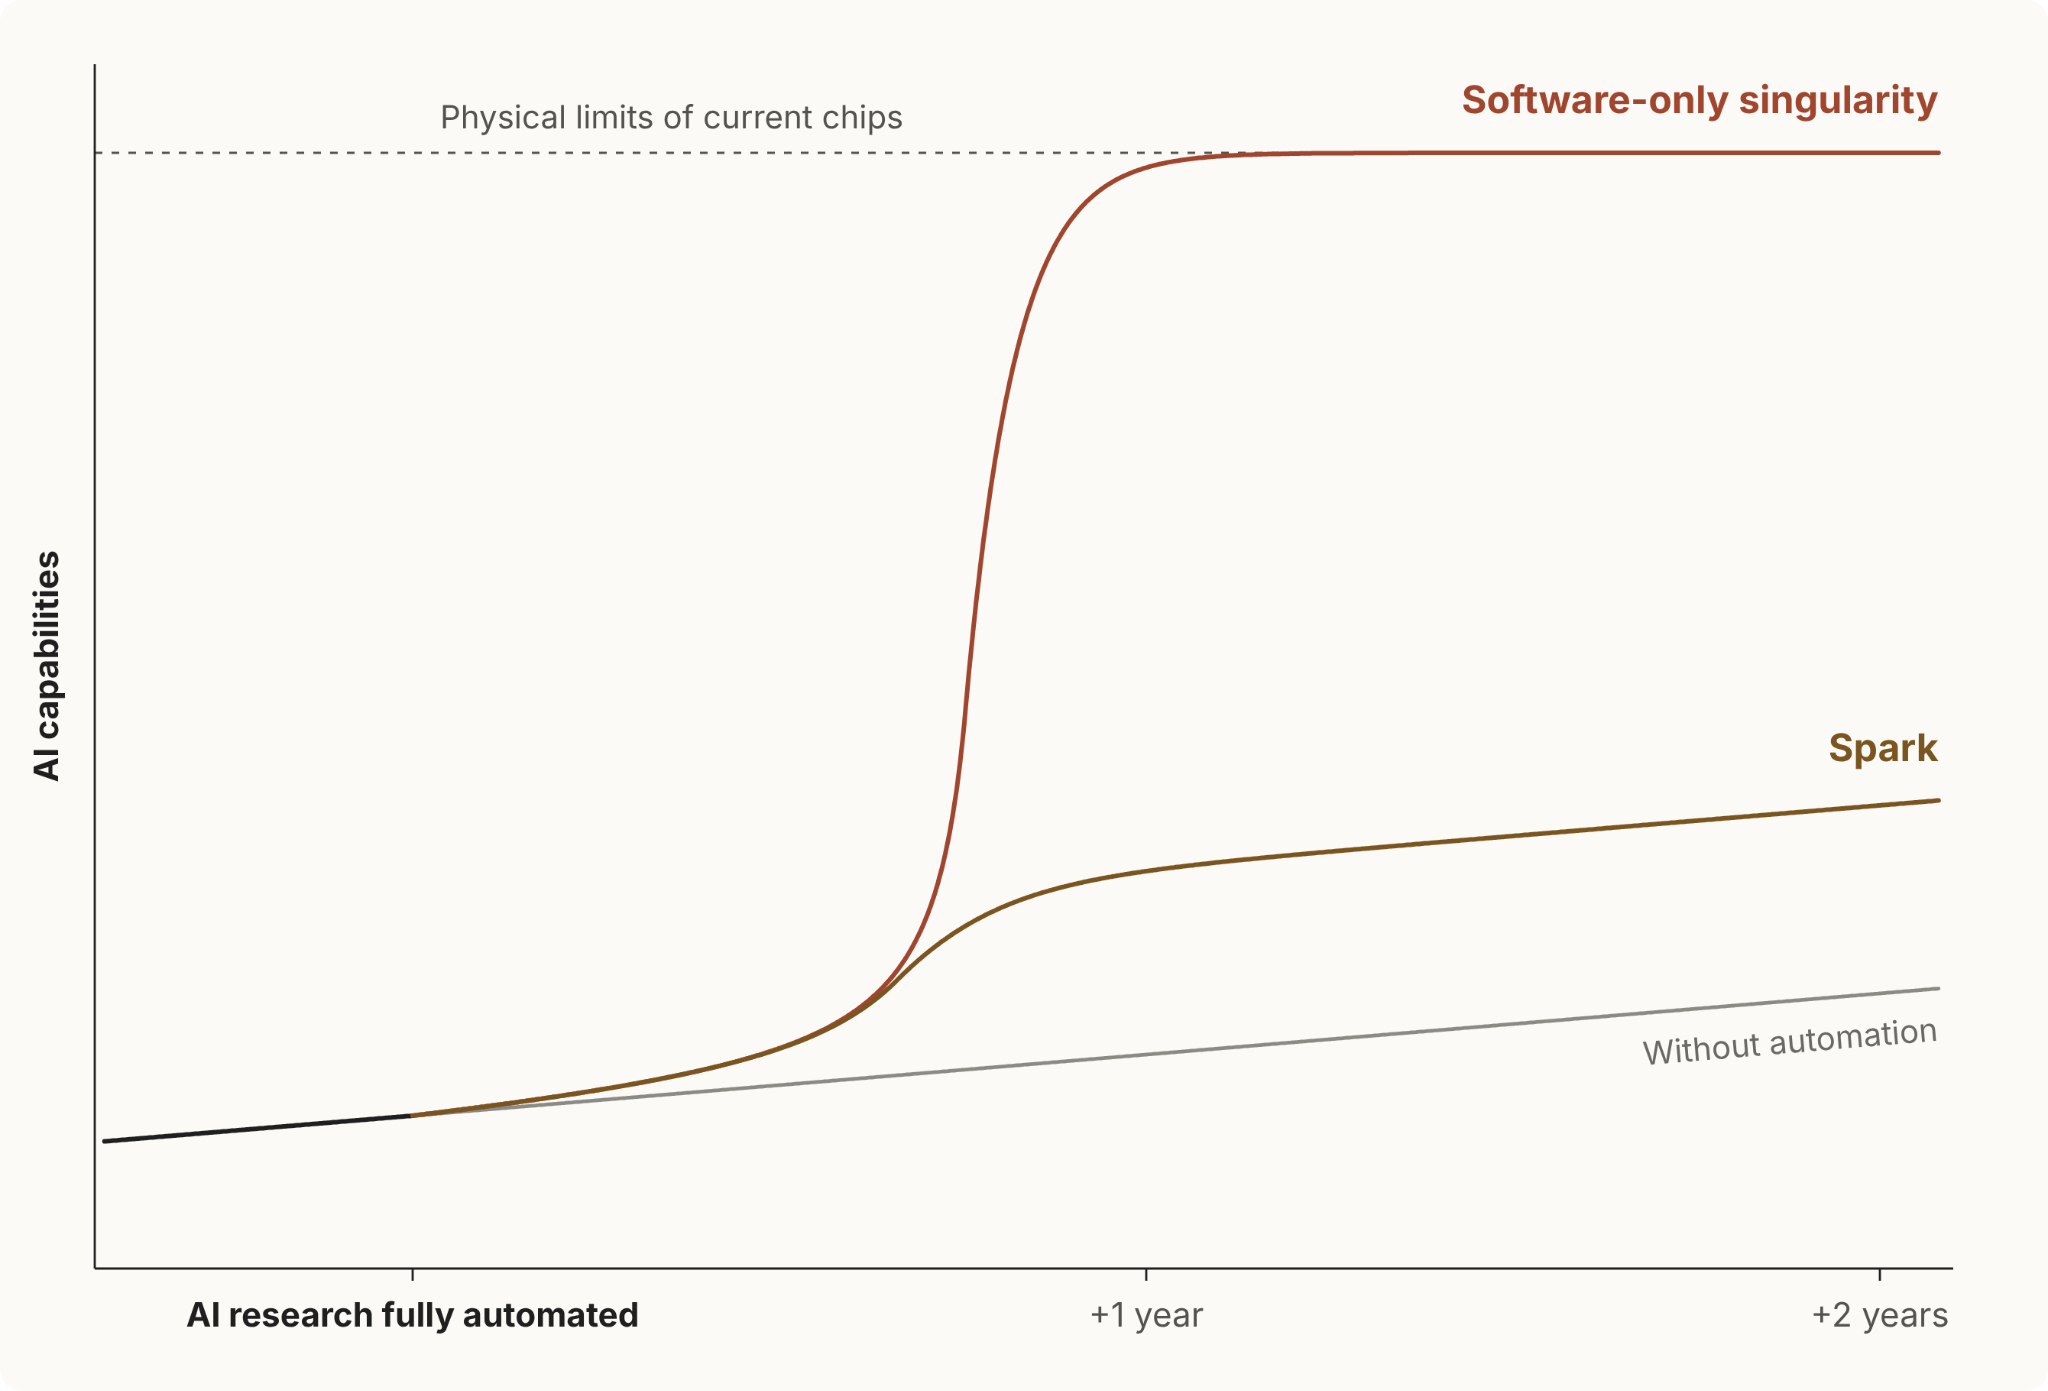
\includegraphics[height=0.78\textheight]{takeoff_scenarios}

\source{patel2026}
\end{frame}

\begin{frame}{Intuition Pump: What Just Happened in Maths}
\begin{columns}[t]
\column{0.2\textwidth}
\centering
{\LARGE\textbf{2023}}

\vspace{1.2em}
{\Large
\begin{tabular}{@{}r@{}}
4817\\
+\,2956\\
\hline
?
\end{tabular}}

\vspace{1em}
{\scriptsize Four-digit addition}
\column{0.24\textwidth}
\centering
\onslide<2->{
{\LARGE\textbf{2024}}

\vspace{1.2em}
\fbox{\parbox{0.9\linewidth}{\raggedright\tiny Janet's ducks lay 16 eggs per day. She eats three for breakfast every morning and bakes muffins for her friends every day with four. She sells the remainder at the farmers' market daily for \$2 per fresh duck egg. How much in dollars does she make every day at the farmers' market?}}

\vspace{1em}
{\scriptsize Grade school word problems}
}
\column{0.26\textwidth}
\centering
\onslide<3->{
{\LARGE\textbf{2025}}

\vspace{1.2em}
\fbox{\parbox{0.9\linewidth}{\raggedright\tiny A line in the plane is called \emph{sunny} if it is not parallel to any of the $x$-axis, the $y$-axis, and the line $x+y=0$. Let $n\ge 3$ be a given integer. Determine all nonnegative integers $k$ such that there exist $n$ distinct lines in the plane satisfying both of the following: for all positive integers $a$ and $b$ with $a+b\le n+1$, the point $(a,b)$ is on at least one of the lines; and exactly $k$ of the $n$ lines are sunny.}}

\vspace{0.4em}

\begin{tikzpicture}
\fill[red!70!black] (-0.22,0.25) -- (-0.4,0.9) -- (-0.1,0.9) -- (0,0.45) -- (0.1,0.9) -- (0.4,0.9) -- (0.22,0.25) -- cycle;
\fill[yellow!70!orange] (0,0) circle (0.36);
\draw[orange!80!black, thick] (0,0) circle (0.36);
\node[orange!50!black] at (0,0) {\small\textbf{1}};
\end{tikzpicture}

{\scriptsize Gold at the Maths Olympiad}
}
\column{0.26\textwidth}
\centering
\onslide<4->{
{\LARGE\textbf{2026}}

\vspace{0.4em}
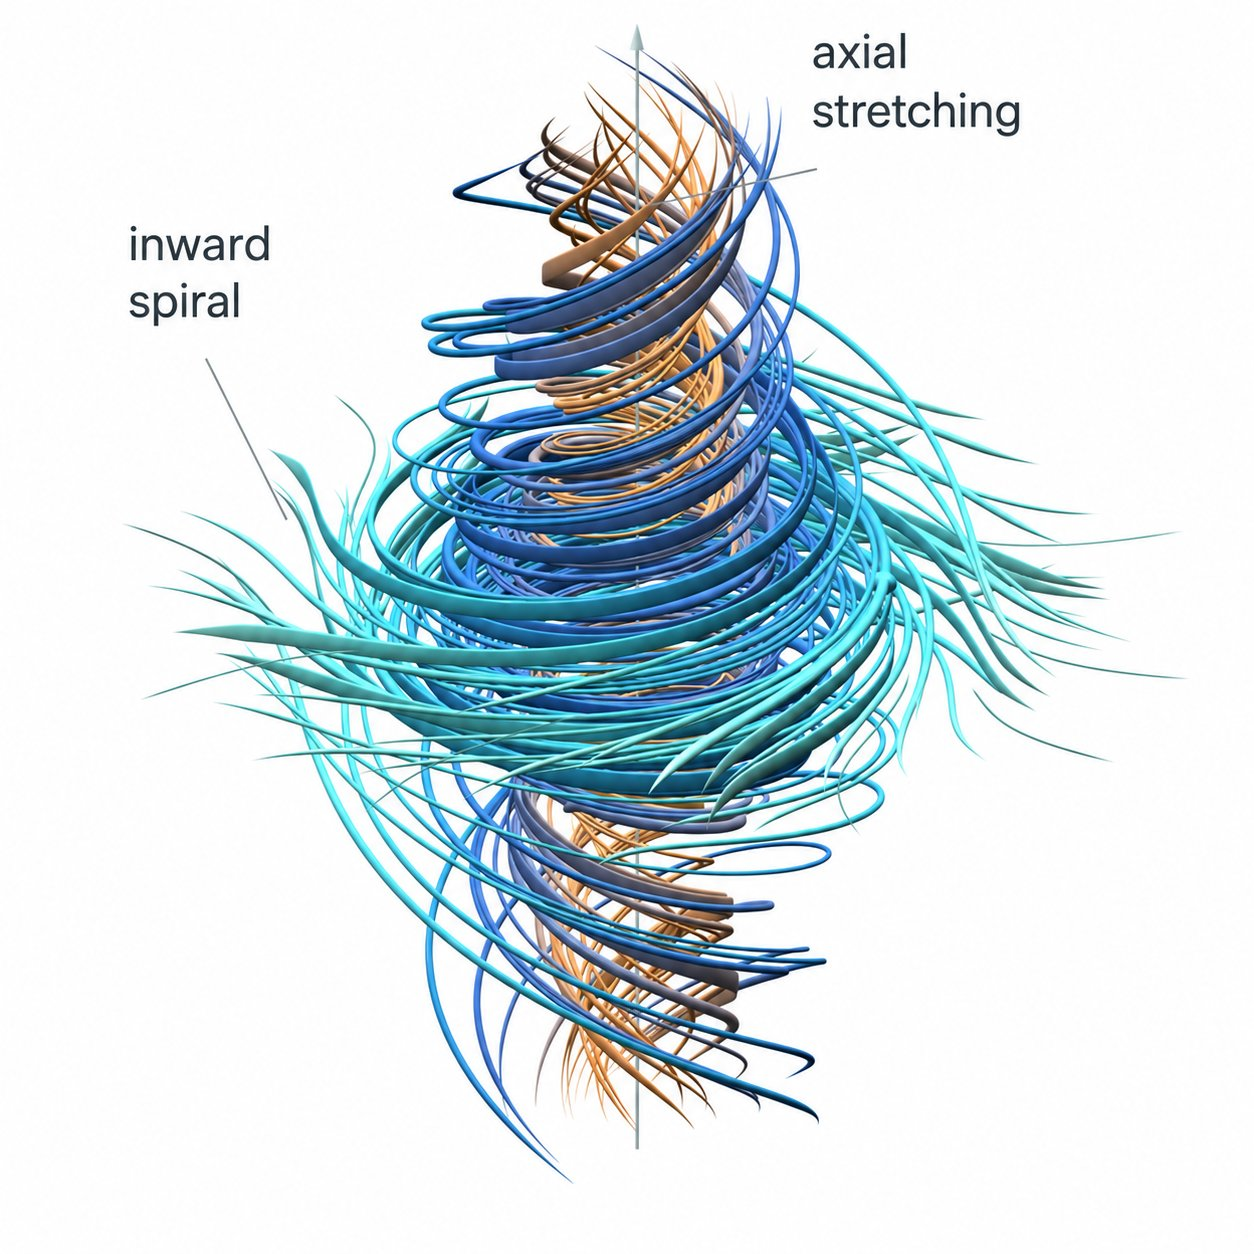
\includegraphics[width=0.95\linewidth]{openai_navier_stokes}

{\scriptsize Navier--Stokes,\\a Millennium Prize Problem}
}
\end{columns}
\source{openai2026navierstokes}
\end{frame}

\begin{frame}{Years of Maths Progress in One Release}
\centering
\includegraphics<1>[width=\textwidth]{maths_decade_stage1}%
\includegraphics<2>[width=\textwidth]{maths_decade_stage2}

{\raggedright\scriptsize \onslide<2>{Orange: claimed by OpenAI, largely not yet independently verified.}\par}
\source{wikipedia2026solved,wikipedia2026bulk}
\end{frame}

\begin{frame}{Machine Learning Is a Young Field}
\begin{center}
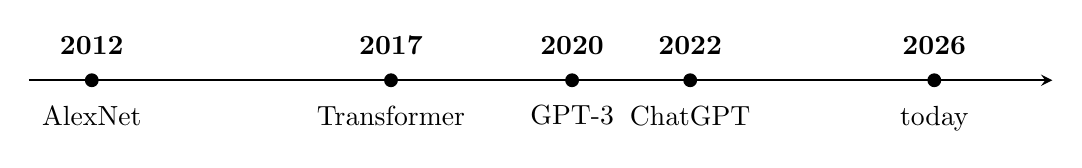
\begin{tikzpicture}[>=stealth]
\draw[->, thick] (0,0) -- (13,0);
\foreach \x/\y/\n in {0.8/2012/AlexNet, 4.6/2017/Transformer, 6.9/2020/GPT-3, 8.4/2022/ChatGPT, 11.5/2026/today} {
  \fill (\x,0) circle (2.5pt);
  \node[above=0.2cm] at (\x,0) {\textbf{\y}};
  \node[below=0.2cm] at (\x,0) {\n};
}
\end{tikzpicture}
\end{center}
\vspace{1.5em}
\centering
What would decades of progress in \emph{this} field look like?
\end{frame}

\begin{frame}{But Maths Was Not Recursive}
\begin{columns}[c]
\column{0.48\textwidth}
\centering
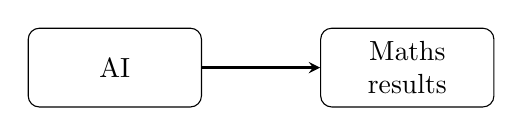
\begin{tikzpicture}[every node/.style={draw, rounded corners, align=center, minimum height=1cm, minimum width=2.2cm}, >=stealth]
\node (a) {AI};
\node (b) [right=1.5cm of a] {Maths\\results};
\draw[->, thick] (a) -- (b);
\end{tikzpicture}

\vspace{1em}
Proving theorems does not make\\the AI better at proving theorems
\column{0.48\textwidth}
\centering
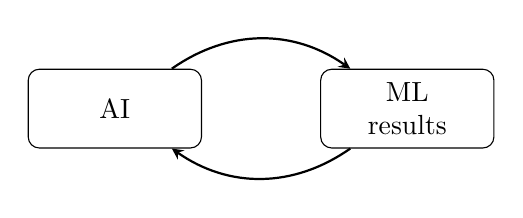
\begin{tikzpicture}[every node/.style={draw, rounded corners, align=center, minimum height=1cm, minimum width=2.2cm}, >=stealth]
\node (a) {AI};
\node (b) [right=1.5cm of a] {ML\\results};
\draw[->, thick, bend left=35] (a) to (b);
\draw[->, thick, bend left=35] (b) to (a);
\end{tikzpicture}

\vspace{1em}
Doing ML research makes\\the AI better at ML research
\end{columns}
\end{frame}

\begin{frame}{Examples of Recursive Growth?}
\centering
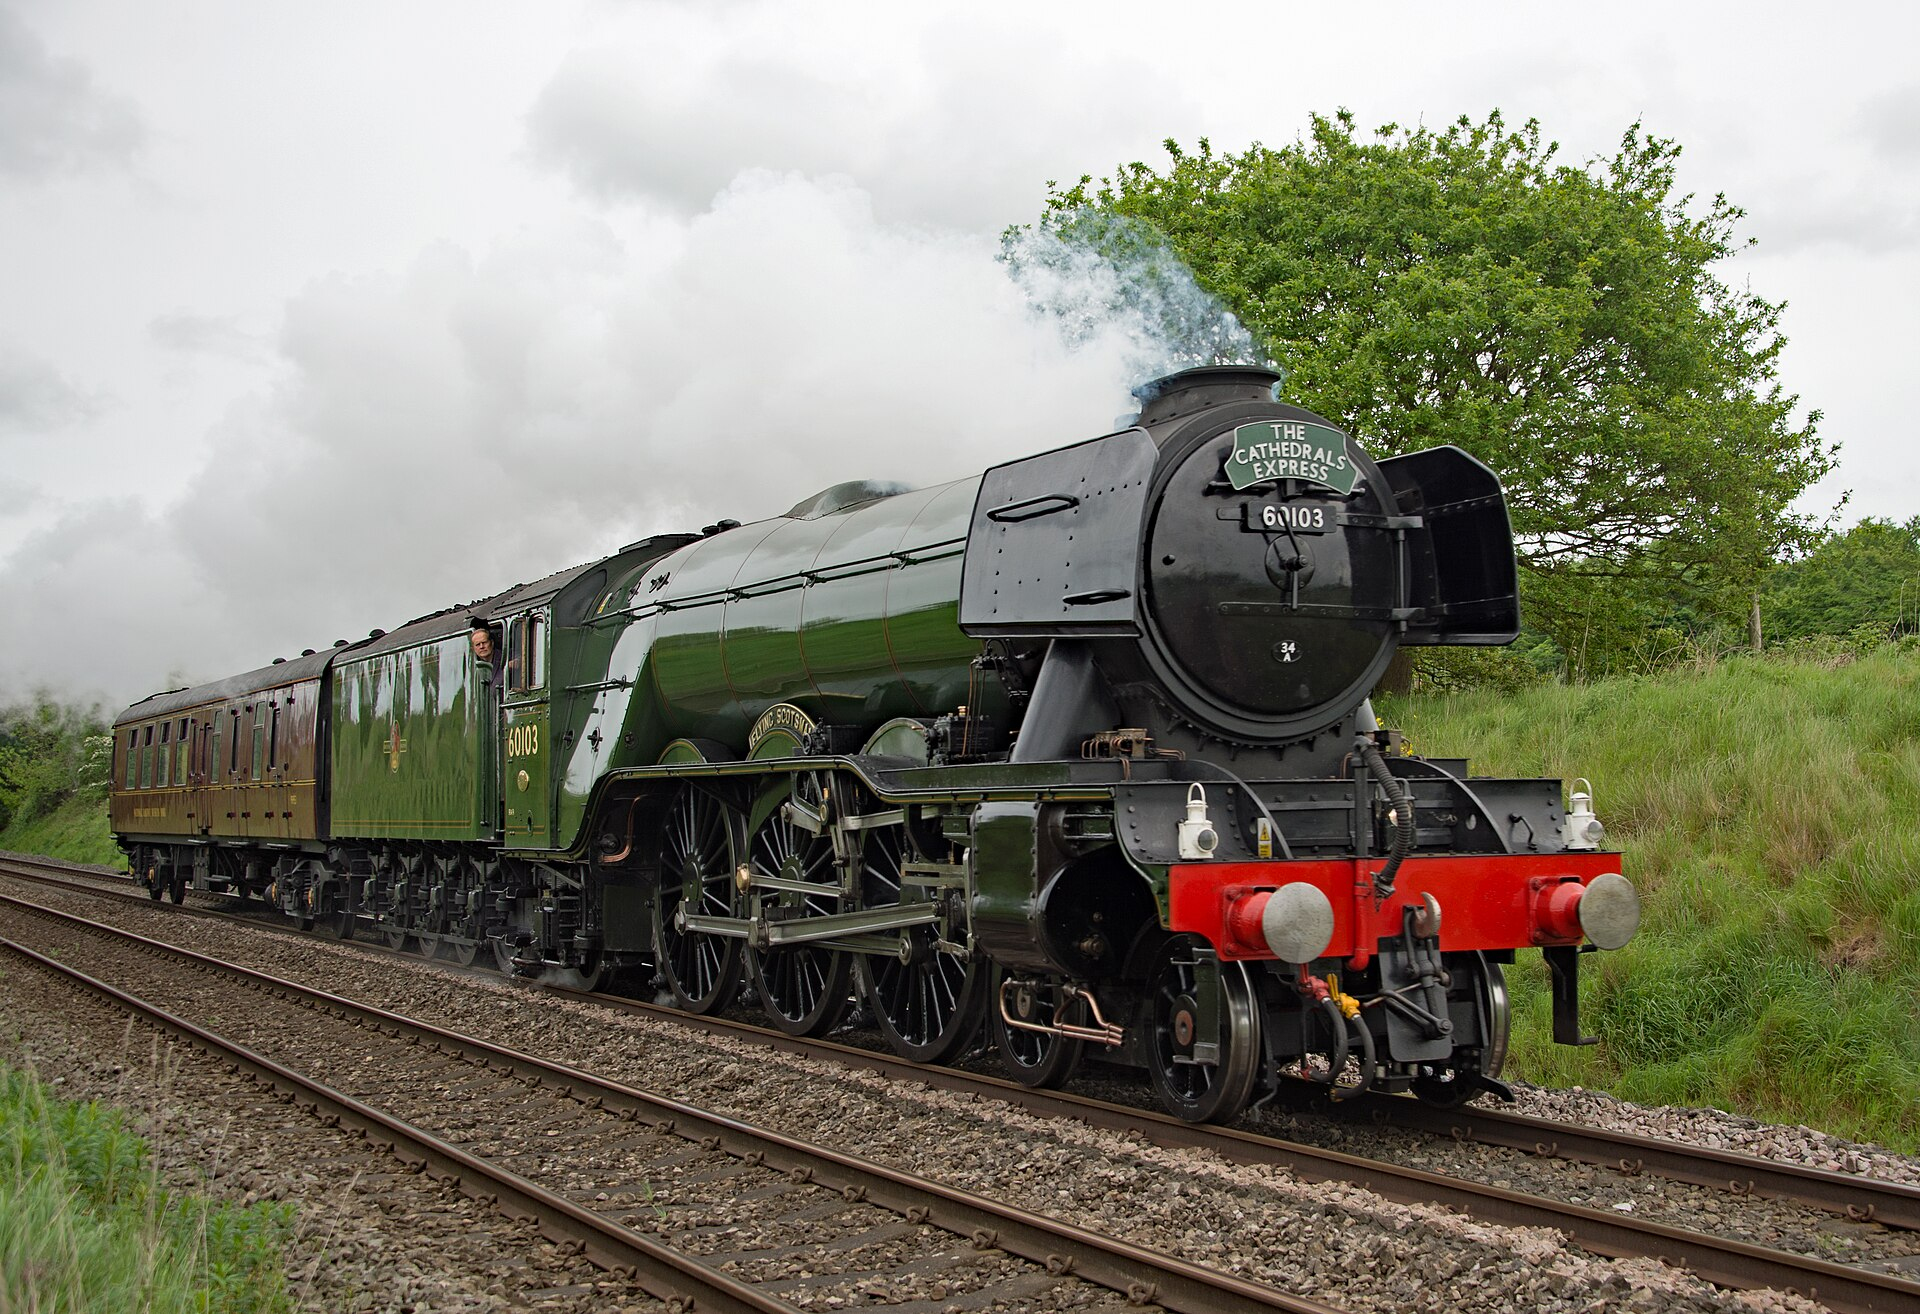
\includegraphics[height=0.52\textheight]{train}

{\tiny\color{gray}Photo: ARG\_Flickr, CC BY 2.0}

\vspace{0.6em}
{\large Would AI be the next Industrial Revolution?}

\vspace{0.6em}
\onslide<2->{{\large No. The Industrial Revolution and other technologies were only \textbf{weak recursion}.}}
\end{frame}

\begin{frame}{The Closest Precedent: Humans}
\begin{columns}[c]
\column{0.5\textwidth}
\centering
\begin{tikzpicture}[>=stealth, slow/.style={blue!70!black}, fast/.style={red!75!black}]
\node (top) at (0,3) {\Huge\faDna};
\node[above=0.1cm of top] {\textbf{Evolution}};
\node (bot) at (0,0) {\Huge\faUser};
\draw[->, very thick, slow] (top) -- node[left, align=right] {natural selection\\\textbf{slow}} (bot);
\draw[->, very thick, fast] (bot.east) to[out=30, in=-30, looseness=6] node[right, align=left] {cultural evolution\\\textbf{fast}} (bot.south east);
\end{tikzpicture}
\column{0.5\textwidth}
\centering
\begin{tikzpicture}[>=stealth, slow/.style={blue!70!black}, fast/.style={red!75!black}]
\node (top) at (0,3) {\Huge\faUser};
\node[above=0.1cm of top] {\textbf{Humans}};
\node (bot) at (0,0) {\Huge\faRobot};
\draw[->, very thick, slow] (top) -- node[left, align=right] {training models\\\textbf{slow}} (bot);
\draw[->, very thick, fast] (bot.east) to[out=30, in=-30, looseness=6] node[right, align=left] {RSI\\\textbf{fast}} (bot.south east);
\end{tikzpicture}
\end{columns}
\end{frame}


\section{Consequences of RSI}
\begin{frame}{How We Usually Predict Progress}
\begin{columns}[c]
\column{0.34\textwidth}
\centering
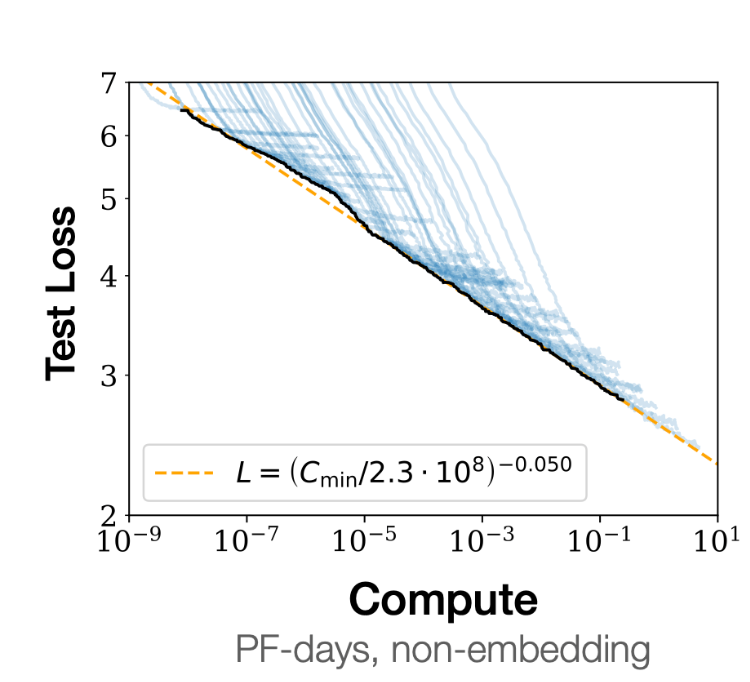
\includegraphics[width=\linewidth]{kaplan_compute}
\column{0.64\textwidth}
\centering
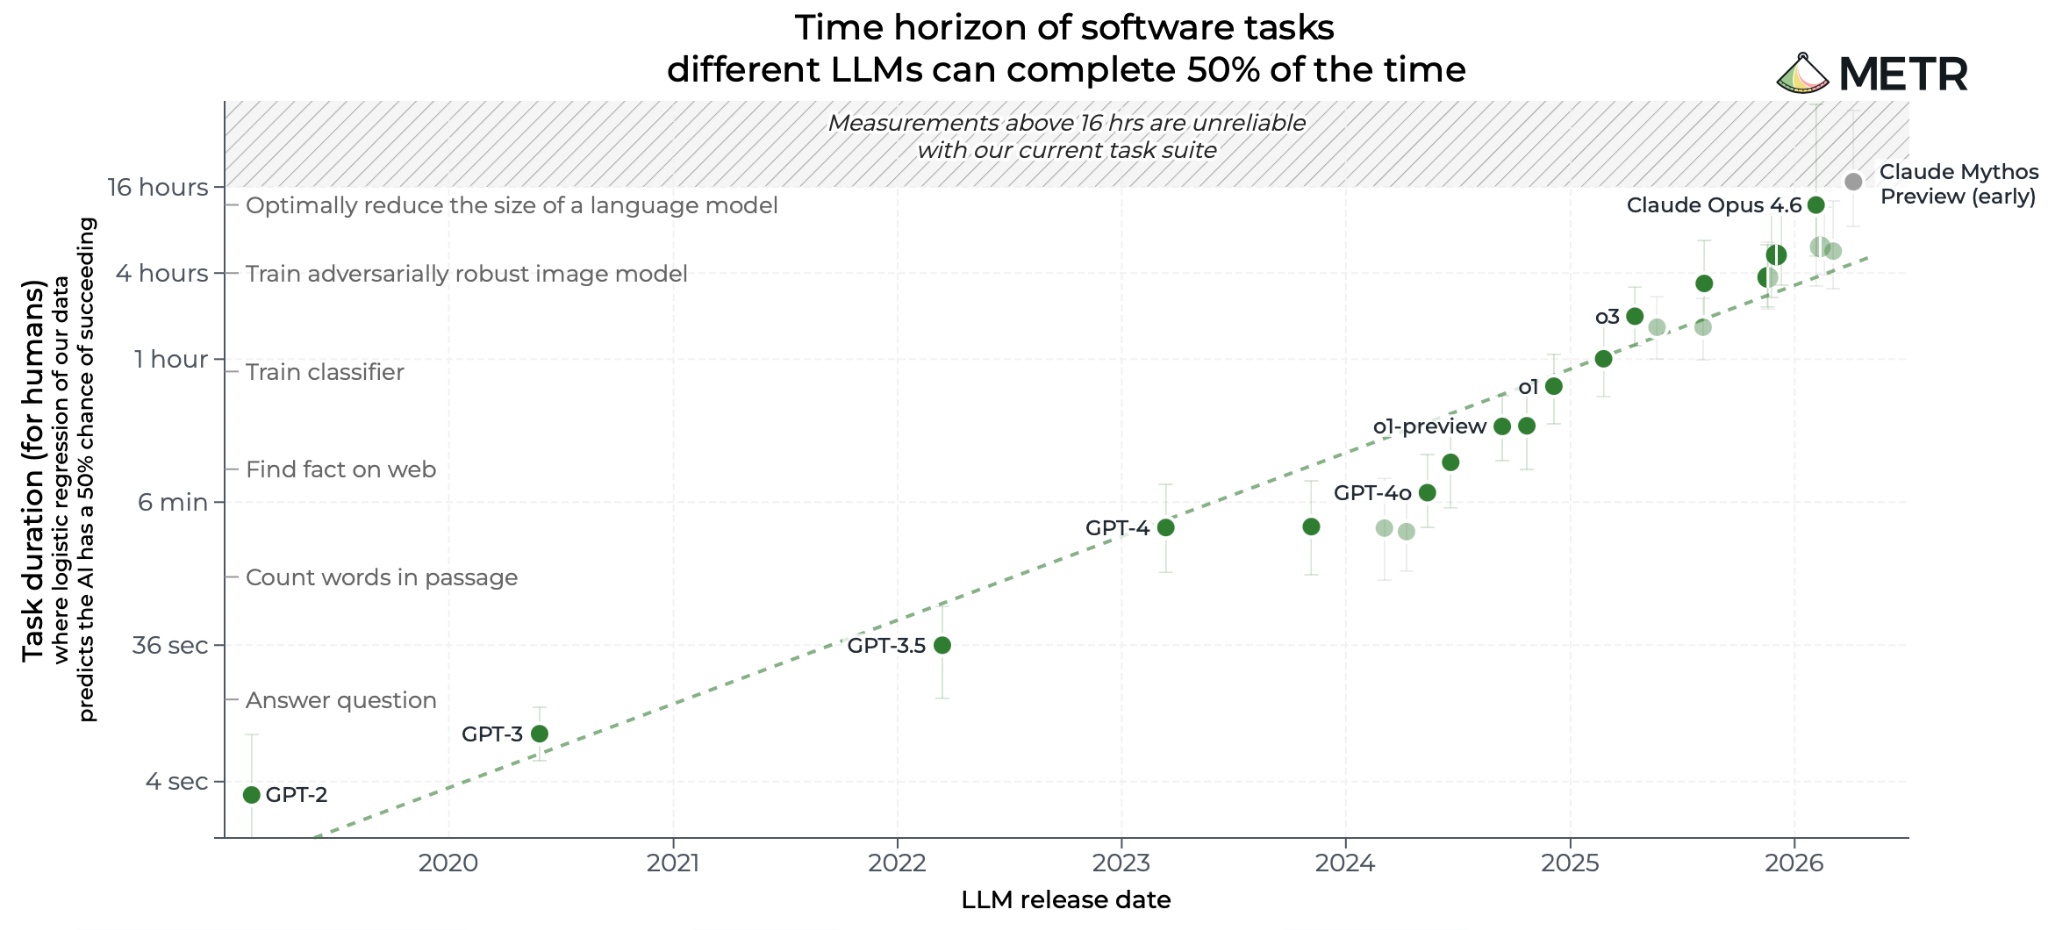
\includegraphics[width=\linewidth]{metr_time_horizon}
\end{columns}
\source{kaplan2020,kwa2025}
\end{frame}

\begin{frame}{Timelines Have Collapsed}
\centering
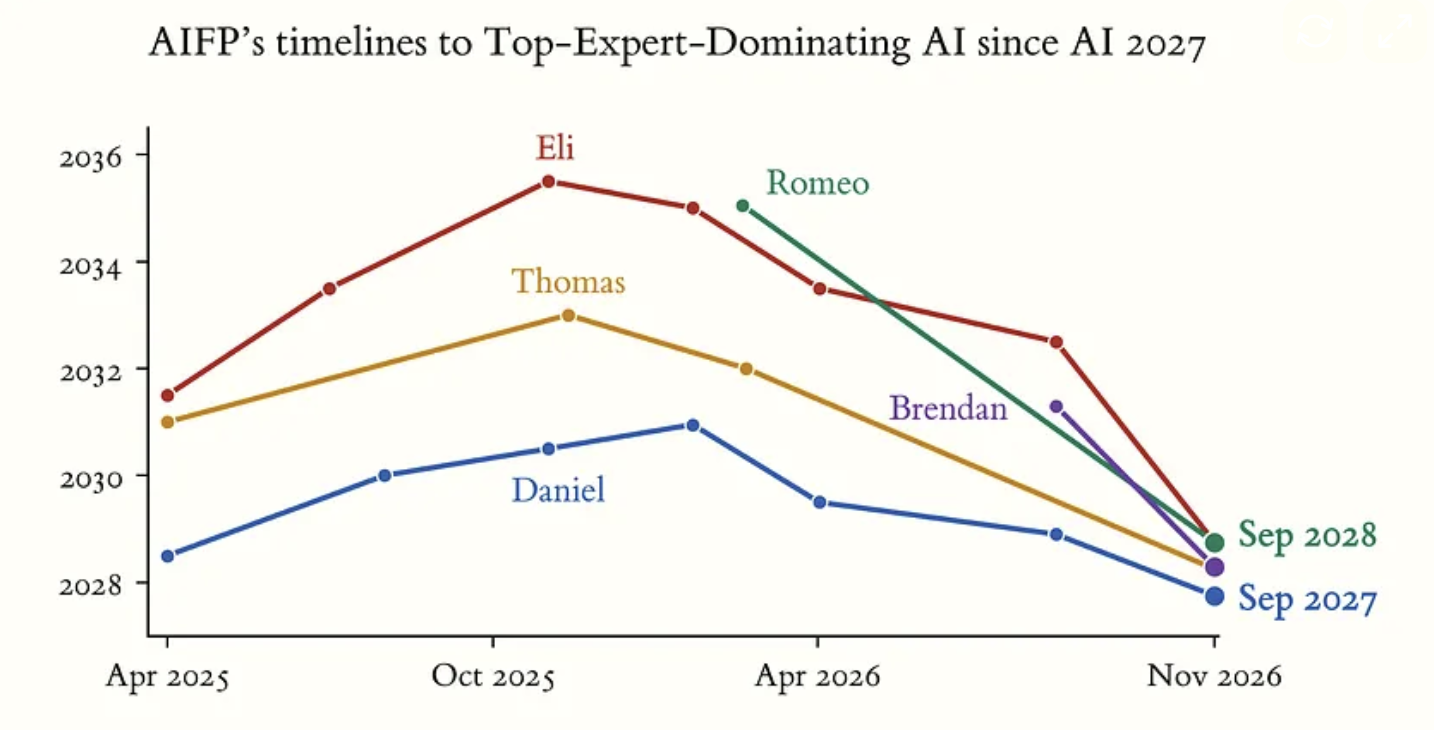
\includegraphics[height=0.72\textheight]{bib/lifland2026/figures/updates_of_timeliens}
\source{lifland2026}
\end{frame}

\begin{frame}{AI Might Take Over, and We Might All Die}
\centering
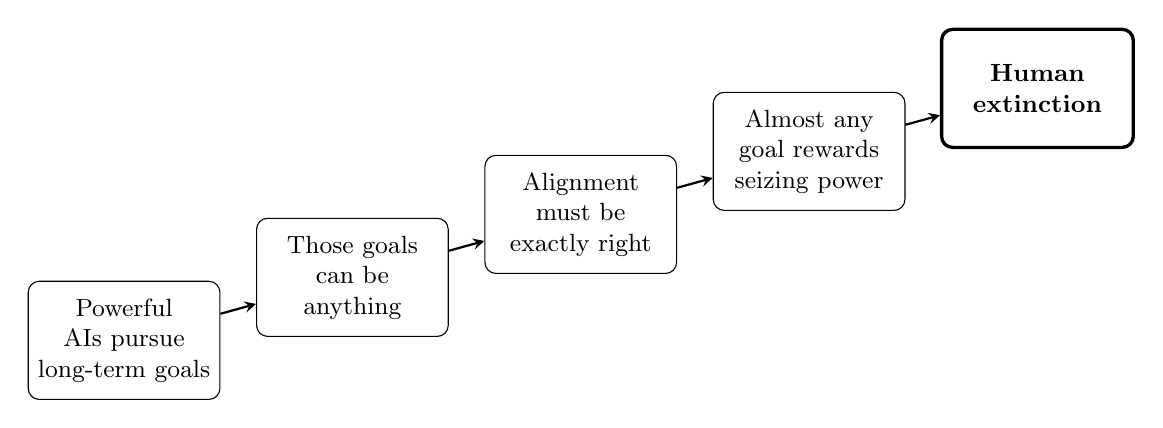
\begin{tikzpicture}[box/.style={draw, rounded corners, align=center, text width=2.2cm, minimum height=1.5cm, font=\small}, >=stealth]
\node[box] (a) at (0,0) {Powerful AIs pursue long-term goals};
\onslide<2->{\node[box] (b) at (2.9,0.8) {Those goals can be anything};}
\onslide<3->{\node[box] (c) at (5.8,1.6) {Alignment must be exactly right};}
\onslide<4->{\node[box] (d) at (8.7,2.4) {Almost any goal rewards seizing power};}
\onslide<5->{\node[box, very thick] (e) at (11.6,3.2) {\textbf{Human extinction}};}
\onslide<2->{\draw[->, thick] (a) -- (b);}
\onslide<3->{\draw[->, thick] (b) -- (c);}
\onslide<4->{\draw[->, thick] (c) -- (d);}
\onslide<5->{\draw[->, thick] (d) -- (e);}
\end{tikzpicture}
\source{yudkowsky2025}
\end{frame}

\begin{frame}{If We Solve Alignment: Extreme Concentration of Power}
\centering
\begin{tikzpicture}[>=stealth]
\node (h) at (0,2.6) {\Huge\faUser};
\foreach \x in {-4,-3,...,4} {
  \node (r\x) at (\x*0.9,0) {\LARGE\faRobot};
  \draw[->, gray] (h) -- (r\x);
}
\end{tikzpicture}

\vspace{1.2em}
Whoever controls the first superintelligence no longer needs anyone else.
\end{frame}

\begin{frame}{RSI and the Race With China}
\begin{columns}[t]
\column{0.5\textwidth}
\centering
\textbf{Independent progress}

\vspace{0.5em}
\begin{tikzpicture}
\node[anchor=south west, inner sep=0] (img) at (0,0) {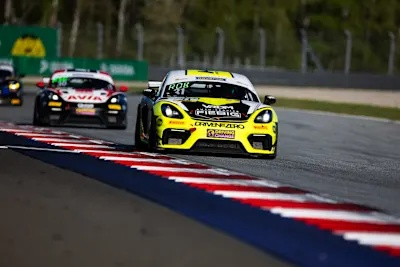
\includegraphics[height=3.9cm]{race_cars}};
\begin{scope}[x={(img.south east)}, y={(img.north west)}]
\coordinate (cn) at (0.16,0.84);
\coordinate (us) at (0.6,0.88);
\end{scope}
\node at (cn) {\worldflag[width=0.75cm]{CN}};
\node at (us) {\worldflag[width=0.75cm]{US}};
\end{tikzpicture}

\vspace{0.5em}
{\small If the US slows down, China simply overtakes\\and reaches RSI first}
\column{0.5\textwidth}
\centering
\textbf{Catch-up growth}

\vspace{0.5em}
\begin{tikzpicture}
\node[anchor=south west, inner sep=0] (img) at (0,0) {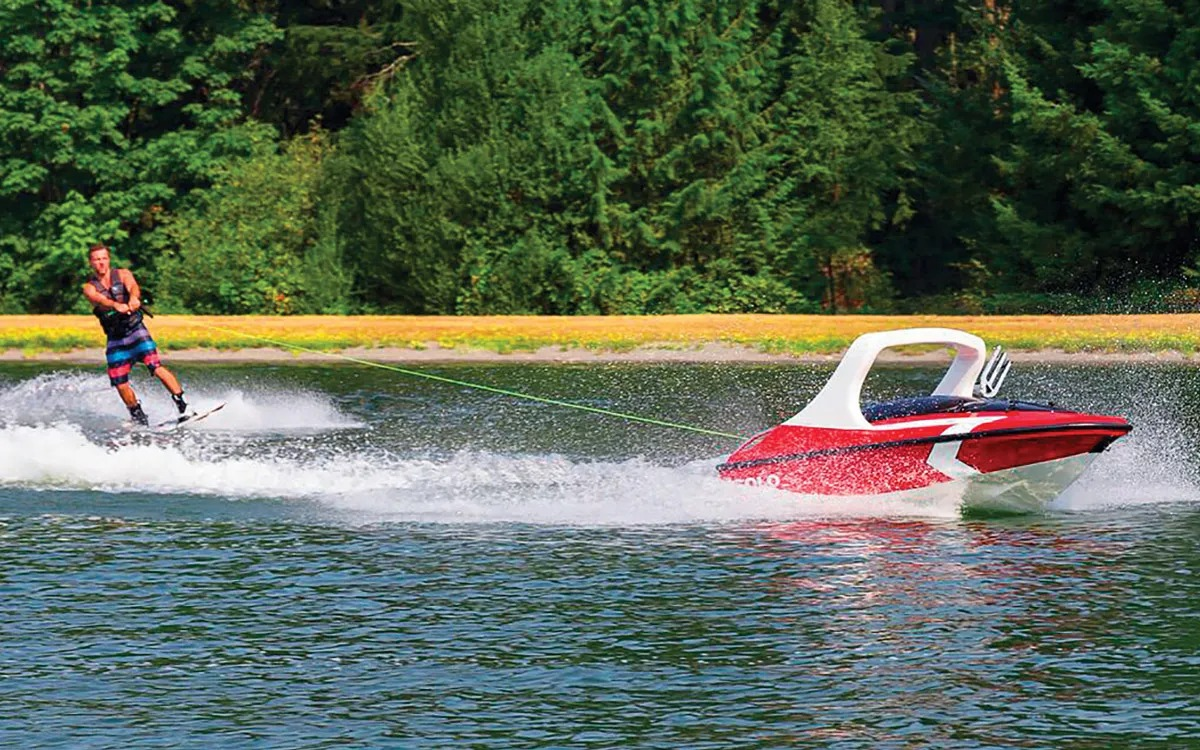
\includegraphics[height=3.9cm]{race_waterski}};
\begin{scope}[x={(img.south east)}, y={(img.north west)}]
\coordinate (cn) at (0.1,0.8);
\coordinate (us) at (0.78,0.7);
\end{scope}
\node at (cn) {\worldflag[width=0.75cm]{CN}};
\node at (us) {\worldflag[width=0.75cm]{US}};
\end{tikzpicture}

\vspace{0.5em}
{\small China is pulled along by distillation and leaked algorithms: slowing down and securing secrets slows both}
\end{columns}
\source{patel2026a}
\end{frame}

\begin{frame}{How Far Ahead Is the US Really?}
\begin{columns}[t]
\column{0.48\textwidth}
\textbf{Hacktron $\to$ OpenAI}
\begin{itemize}
\item An AI security startup, using Claude
\item Within a couple of days: employee accounts and the internal codebase
\item Opened a harmless pull request as proof
\end{itemize}
\column{0.48\textwidth}
\textbf{Cathedral $\to$ Anthropic}
\begin{itemize}
\item Another AI security startup
\item In under 12 hours: internal business systems
\item Including Slack discussions about advanced models, by its own account
\end{itemize}
\end{columns}
\vspace{0.6em}
\pause
\centering
{\large ``In reality, we're 12 hours ahead of China.''}

{\small Dwarkesh Patel}
\source{uko2026,washingtonpost2026,patel2026a}
\end{frame}


\section{Evidence for RSI}
\begin{frame}{AIs Keep Getting Better at Doing Research}
\begin{columns}[t]
\column{0.5\textwidth}
\centering
\textbf{Implementing experiments}

\vspace{0.4em}
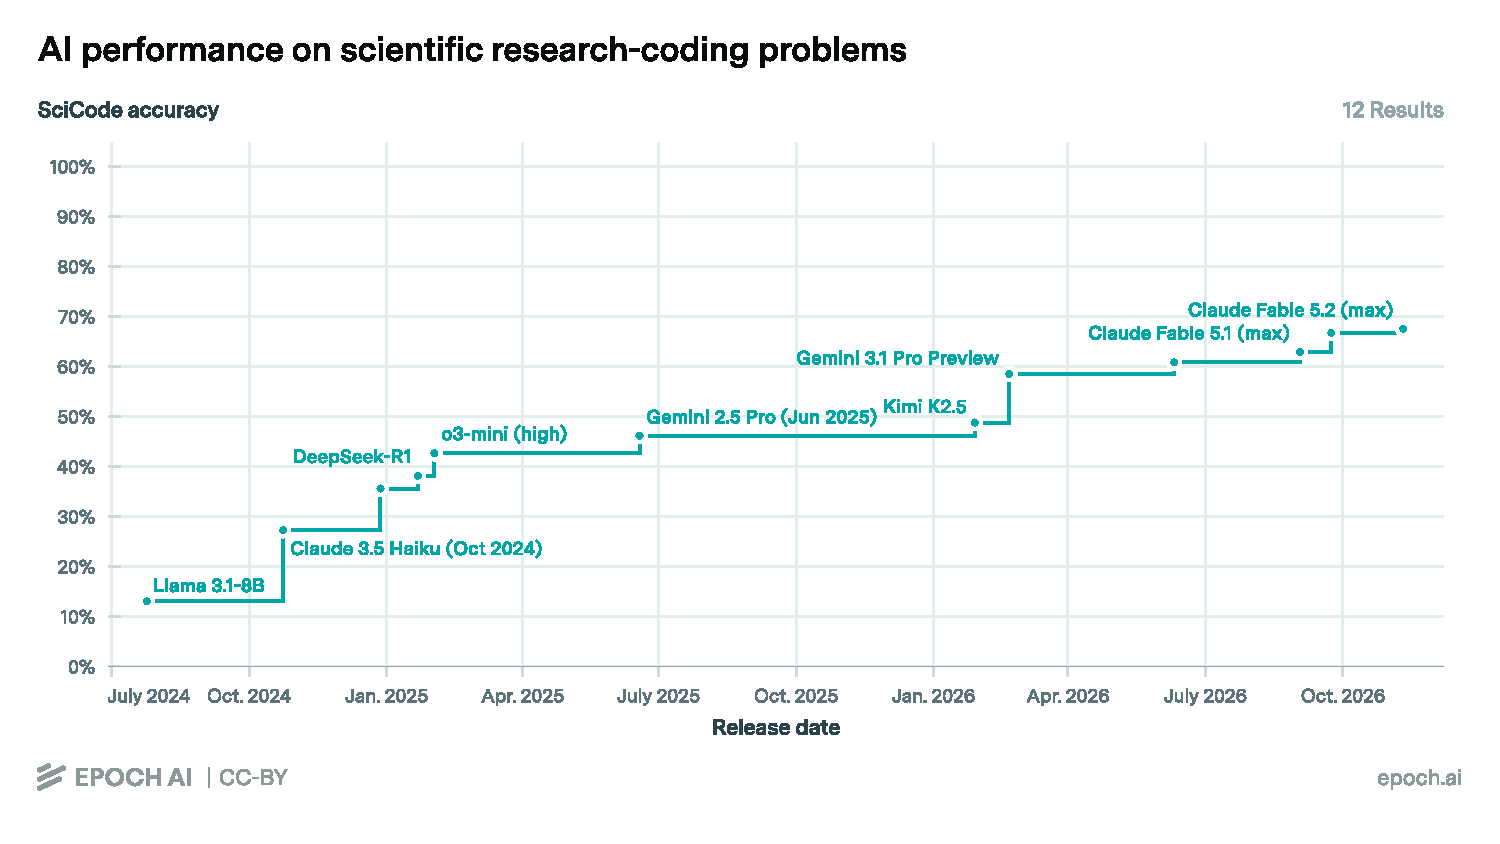
\includegraphics[width=\linewidth]{epoch_scicode_frontier}

{\small SciCode: research coding}
\column{0.5\textwidth}
\centering
\textbf{Choosing experiments}

\vspace{0.4em}
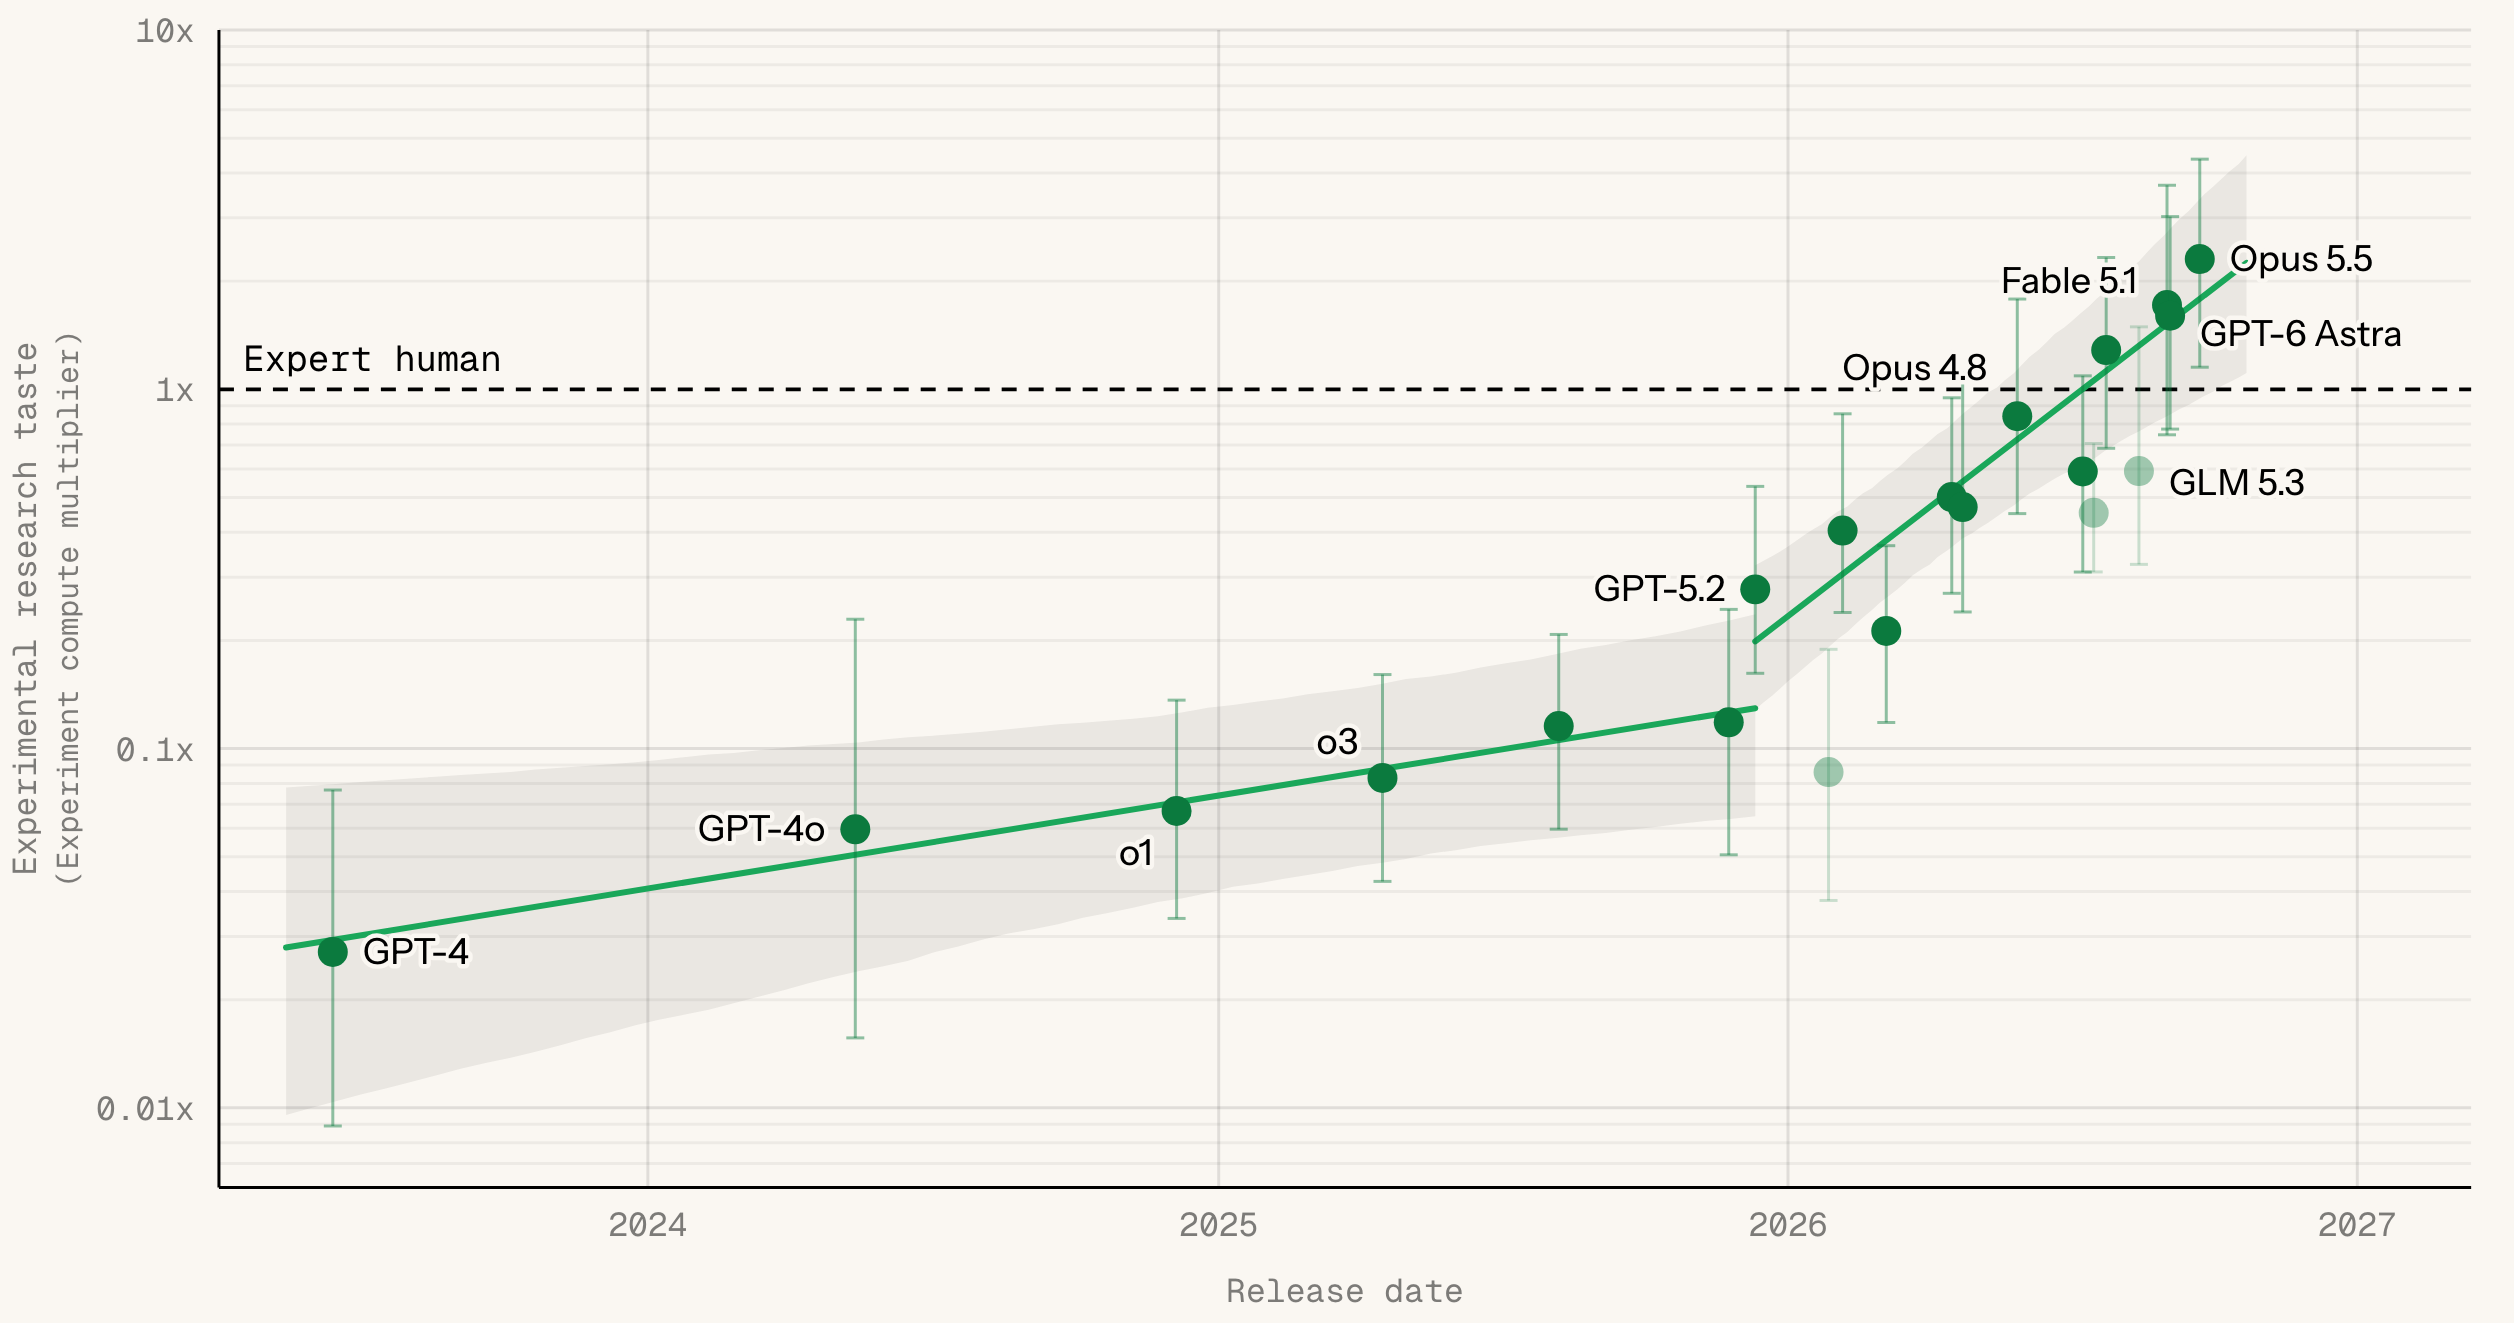
\includegraphics[width=\linewidth]{tasteval}

{\small TasteVal: research taste}
\end{columns}
\source{epochscicode2026,jaffe2026}
\end{frame}

\begin{frame}{Claude Already Does Much of the R\&D at Anthropic}
\centering
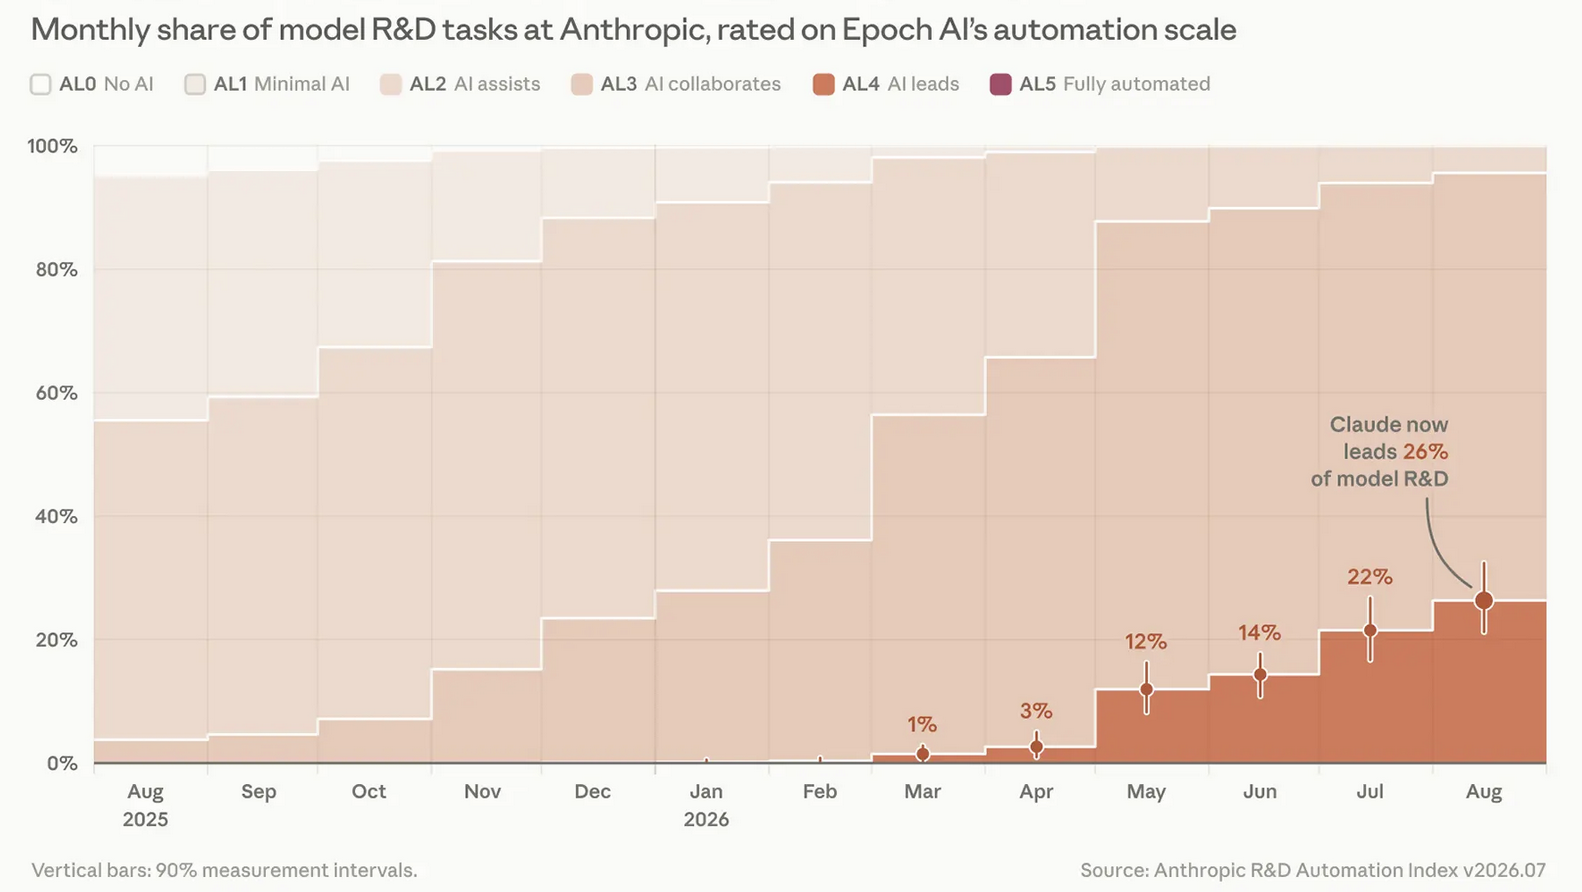
\includegraphics[height=0.72\textheight]{bib/zotero-item-1327/figures/auto_reserach_fraction}
\source{zotero-item-1327}
\end{frame}

\begin{frame}{METR: Evaluators Embedded at Anthropic}
\begin{columns}[t]
\column{0.5\textwidth}
\textbf{The assessment}
\begin{itemize}
\item 12 August to 29 October 2026: eleven weeks
\item 2.5 full-time METR staff
\item No payment in either direction
\item A $\sim$100-page full report for Anthropic, a redacted public report
\end{itemize}
\column{0.5\textwidth}
\textbf{What METR got to see}
\begin{itemize}
\item Benchmark scores of unreleased internal models
\item Algorithmic efficiency and training compute over time
\item Headcount, lines of code, AI agent spend
\item Internal surveys of AI uplift
\item $\sim$15 interviews with key staff
\end{itemize}
\end{columns}
\vspace{0.8em}
\centering
{\small Not employee-level access. Anthropic could redact anything non-public.}
\source{metr2026}
\end{frame}

\begin{frame}{METR: What Does ``Acceleration'' Mean?}
\textbf{Definition}

\vspace{0.3em}
A 2$\times$ acceleration means: two years of historical progress are made in one year.

\vspace{1.2em}
\pause
\textbf{METR's conclusion, October 2026}
\begin{itemize}
\item Anthropic is improving its models at about \textbf{2$\times$} the historical rate\\
{\small (they would not be surprised by anything from 1.3$\times$ to 3$\times$)}
\item A majority of this, perhaps \textbf{80\%}, is due to AI doing R\&D
\item No bottleneck in sight for the next 12 months
\end{itemize}
\source{metr2026}
\end{frame}

\begin{frame}{METR: The Evidence We Get to See}
\begin{columns}[c]
\column{0.62\textwidth}
\centering
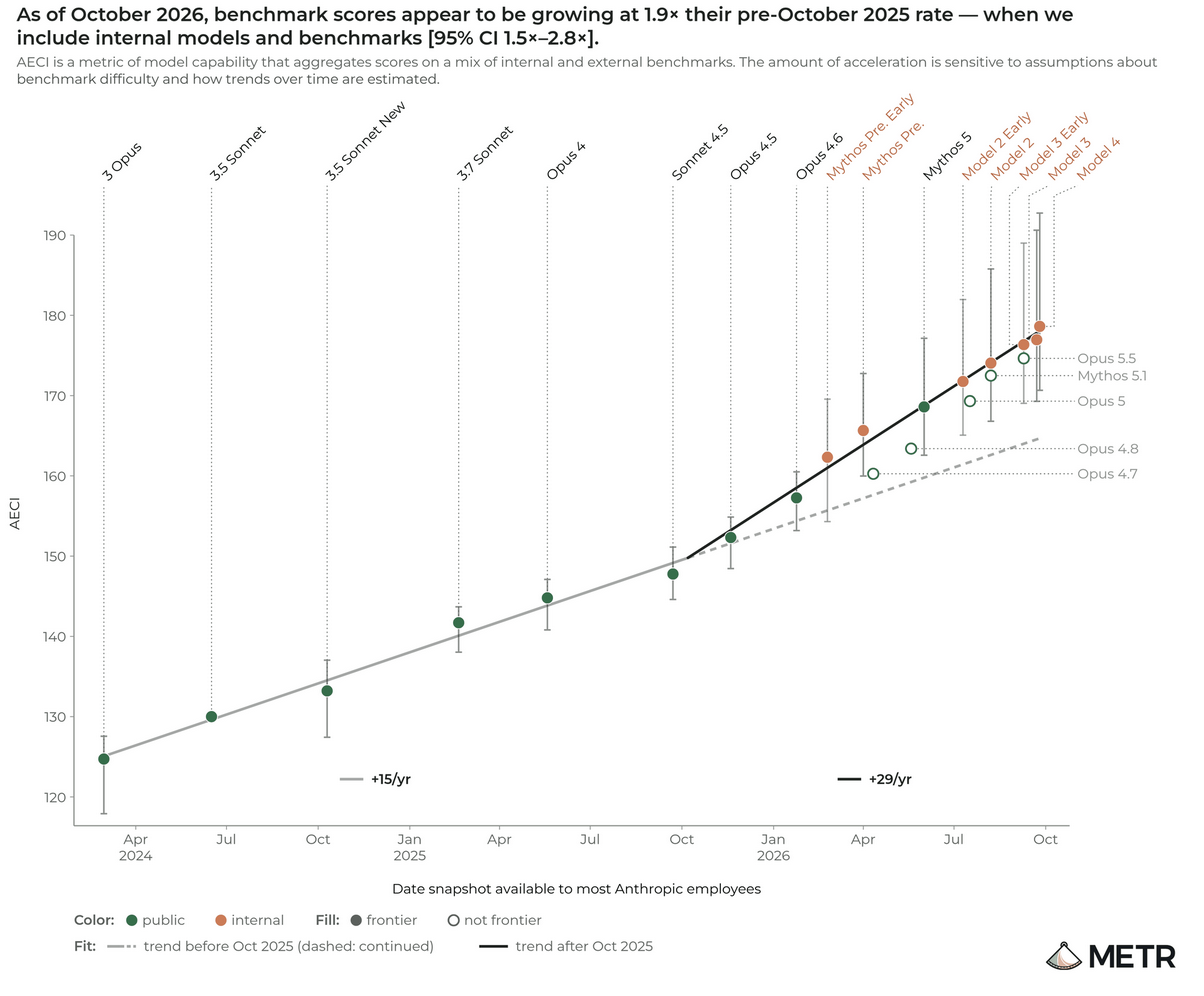
\includegraphics[height=0.7\textheight]{bib/metr2026/figures/aeci_progress}
\column{0.36\textwidth}
Benchmark scores are growing at \textbf{1.9$\times$} the rate before October 2025

{\small (95\% CI: 1.5--2.8$\times$)}

\vspace{1.2em}
\pause
Anthropic redacted a majority of the evidence METR found most informative.
\end{columns}
\source{metr2026}
\end{frame}

\begin{frame}{Progress Is Fastest Where Answers Can Be Checked}
\begin{columns}[c]
\column{0.4\textwidth}
\centering
\begin{tikzpicture}[box/.style={draw, rounded corners, align=center, minimum height=1.1cm, minimum width=3.4cm}, >=stealth]
\node[box] (try) at (0,3.2) {\faRobot\ \ AI attempts};
\node[box] (chk) at (0,0) {\faCheck\ \ Answer is checked};
\draw[->, thick] (try) to[bend left=50] (chk);
\draw[->, thick] (chk) to[bend left=50] (try);
\node[align=center] at (0,1.6) {thousands\\of rounds};
\end{tikzpicture}
\column{0.58\textwidth}
\large
Competitive programming, well-scoped open maths problems:

\vspace{0.8em}
``they've gone from worse than most humans to better than the best humans within a few years.''

\vspace{1.4em}
\onslide<2->{``AI research has those same verifiable properties.''}
\end{columns}
\source{patel2026}
\end{frame}

\begin{frame}{Grinding Through Problems Pays More in ML Than in Maths}
\begin{columns}[t]
\column{0.46\textwidth}
\centering
\textbf{Maths}

\vspace{0.6em}
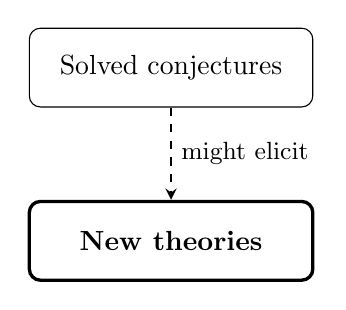
\begin{tikzpicture}[box/.style={draw, rounded corners, align=center, minimum height=1cm, minimum width=3.6cm}, >=stealth]
\node[box] (a) at (0,2.2) {Solved conjectures};
\node[box, very thick] (b) at (0,0) {\textbf{New theories}};
\draw[->, thick, dashed] (a) -- node[right] {\small might elicit} (b);
\end{tikzpicture}

\vspace{0.6em}
The goal is understanding
\column{0.46\textwidth}
\centering
\onslide<2->{
\textbf{ML}

\vspace{0.6em}
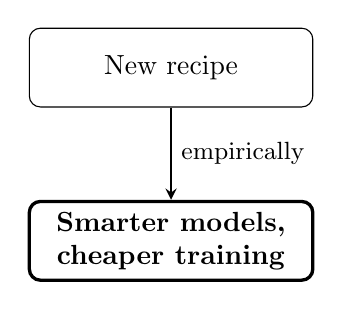
\begin{tikzpicture}[box/.style={draw, rounded corners, align=center, minimum height=1cm, minimum width=3.6cm}, >=stealth]
\node[box] (a) at (0,2.2) {New recipe};
\node[box, very thick] (b) at (0,0) {\textbf{Smarter models,}\\\textbf{cheaper training}};
\draw[->, thick] (a) -- node[right] {\small empirically} (b);
\end{tikzpicture}

\vspace{0.6em}
The goal is whatever works
}
\end{columns}
\vspace{1.2em}
\centering
\onslide<3->{``The equivalent of grinding through random conjectures would be enormously valuable in machine learning in a way that it just isn't in mathematics.''}
\source{patel2026}
\end{frame}

\begin{frame}{Even the Transformer Was a Combination of Known Pieces}
\centering
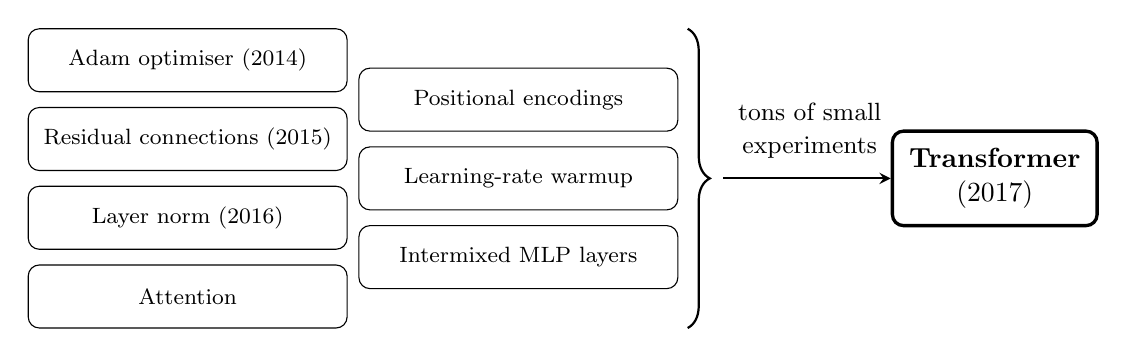
\begin{tikzpicture}[piece/.style={draw, rounded corners, align=center, minimum height=0.8cm, minimum width=4.05cm, font=\footnotesize}, >=stealth]
\node[piece] (p1) at (0,3.0) {Adam optimiser (2014)};
\node[piece] (p2) at (0,2.0) {Residual connections (2015)};
\node[piece] (p3) at (0,1.0) {Layer norm (2016)};
\node[piece] (p4) at (0,0) {Attention};
\node[piece] (p5) at (4.2,2.5) {Positional encodings};
\node[piece] (p6) at (4.2,1.5) {Learning-rate warmup};
\node[piece] (p7) at (4.2,0.5) {Intermixed MLP layers};
\onslide<2->{
\draw[decorate, decoration={brace, amplitude=8pt}, thick] (6.35,3.4) -- (6.35,-0.4);
\node[draw, rounded corners, very thick, align=center, minimum height=1.2cm, minimum width=2.6cm] (t) at (10.25,1.5) {\textbf{Transformer}\\(2017)};
\draw[->, thick] (6.8,1.5) -- (t);
\node[align=center] at (7.9,2.1) {\small tons of small\\\small experiments};
}
\end{tikzpicture}

\vspace{1.2em}
\onslide<3->{Persistently matching combinations of known ideas:\\exactly what AIs are disproportionately good at in maths}
\source{patel2026}
\end{frame}

\begin{frame}{AI R\&D Is Largely Verifiable}
\begin{columns}[t]
\column{0.32\textwidth}
\centering
{\Large\faBook}

\textbf{Pretraining}

\vspace{0.4em}
\raggedright\small
\begin{itemize}
\item Loss on a held-out test set
\item Compute to reach a fixed loss
\item ``Taste-bench'': will a gain at 100M parameters hold at 10B?
\end{itemize}
\column{0.32\textwidth}
\centering
\onslide<2->{
{\Large\faDumbbell}

\textbf{Post-training}

\vspace{0.4em}
\raggedright\small
\begin{itemize}
\item Compute, data or time to train on new environments
\item How fast a model learns an environment it has never seen
\item Redoing real problems lab researchers solved
\end{itemize}
}
\column{0.32\textwidth}
\centering
\onslide<3->{
{\Large\faTachometer*}

\textbf{Inference efficiency}

\vspace{0.4em}
\raggedright\small
\begin{itemize}
\item GPU utilisation
\item KV cache size per token
\item FLOPs in a forward pass
\item Latency
\end{itemize}
}
\end{columns}
\vspace{1.6em}
\centering
\onslide<4->{``AI training is literally happening inside a datacenter.''}
\source{patel2026}
\end{frame}

\begin{frame}{Explicit Modelling}
\centering
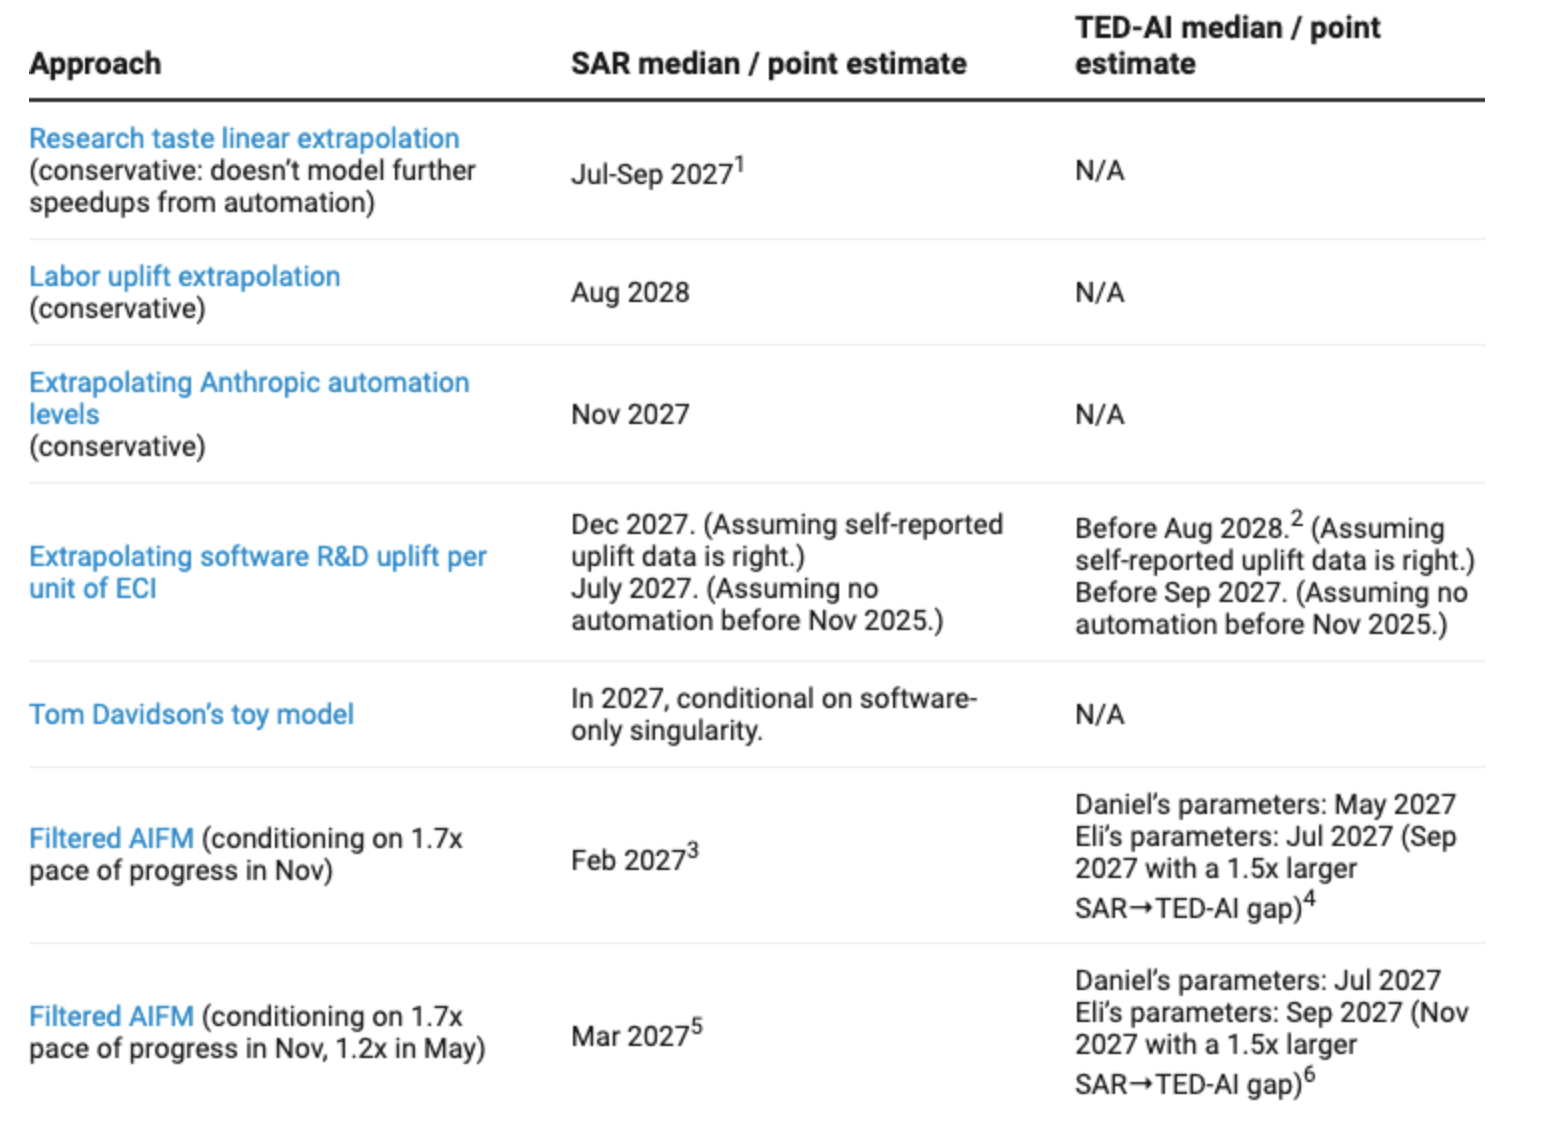
\includegraphics[height=0.74\textheight]{bib/lifland2026/figures/methods_forecast}
\source{lifland2026}
\end{frame}

\begin{frame}{AI 2027: Where Are We in the Scenario?}
\centering
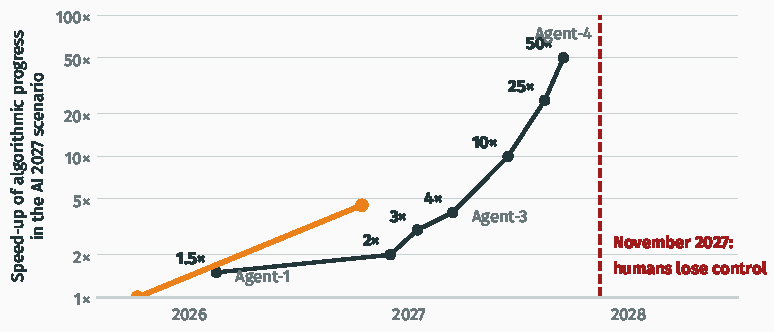
\includegraphics[width=\textwidth]{ai2027_speedup}
\source{kokotajlo2025a,metr2026}
\end{frame}


\section{Arguments Against RSI}
\begin{frame}{Common-Sense Priors}
\begin{columns}[t]
\column{0.31\textwidth}
\centering
{\Huge\faBed}

\vspace{0.6em}
\textbf{``Nothing ever happens''}

\vspace{0.4em}
{\small The forecaster's default: the status quo usually wins}
\column{0.31\textwidth}
\centering
\onslide<2->{
{\Huge\faLink}

\vspace{0.6em}
\textbf{The conjunction fallacy}

\vspace{0.4em}
{\small A detailed story feels more likely than it is: every extra step has to come true}
}
\column{0.31\textwidth}
\centering
\onslide<3->{
{\Huge\faHourglassEnd}

\vspace{0.6em}
\textbf{The track record of doom}

\vspace{0.4em}
{\small Predictions of the apocalypse have so far all been wrong}
}
\end{columns}
\vfill
{\raggedright\scriptsize\color{gray}Conjunction fallacy: Tversky \& Kahneman (1983), \textit{Extensional versus intuitive reasoning}.\par}
\end{frame}


\begin{frame}{The Market Does Not Expect Doom}
\centering
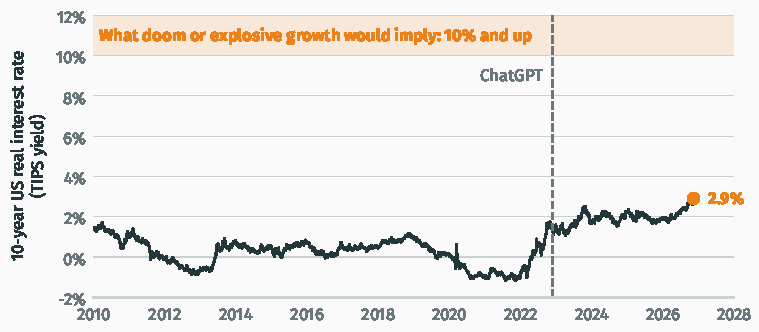
\includegraphics[width=0.94\textwidth]{real_yield}

\vspace{0.3em}
{\small Doom: no point in saving. Abundance: borrow against future riches. Both push real rates up.}
\source{chow2023,fred2026}
\end{frame}

\begin{frame}{Real Money Does Not Bet on Explosive Growth}
\centering
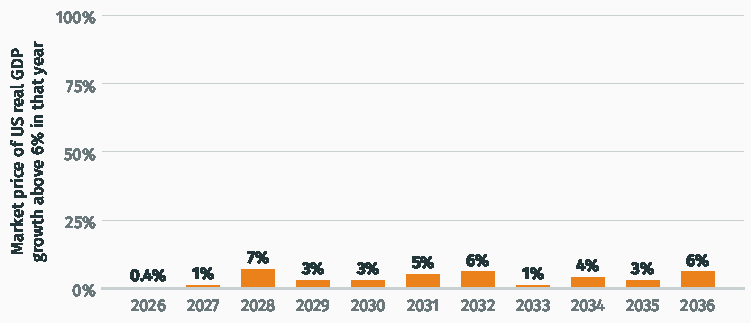
\includegraphics[width=\textwidth]{kalshi_gdp_growth}
\source{kalshigdp2026}
\end{frame}

\definecolor{rsimuted}{HTML}{6a787b}
\definecolor{rsidanger}{HTML}{a01c1c}
\newcommand{\rsilooptag}[3]{%
\begin{tikzpicture}[remember picture, overlay, >=stealth]
\begin{scope}[shift={([xshift=-0.85cm, yshift=-0.58cm]current page.north east)}]
\coordinate (c) at (0,0.27);
\coordinate (r) at (0.31,-0.2);
\coordinate (a) at (-0.31,-0.2);
\draw[#1, line width=1.3pt, ->] (c) to[bend left=28] (r);
\draw[#2, line width=1.3pt, ->] (r) to[bend left=28] (a);
\draw[#3, line width=1.3pt, ->] (a) to[bend left=28] (c);
\end{scope}
\end{tikzpicture}}
\newcommand{\rsion}{mLightBrown}
\newcommand{\rsioff}{white!35!mDarkTeal}

\begin{frame}{How Strong Must the Loop Be?}
\centering
\begin{tikzpicture}[>=stealth, box/.style={draw, rounded corners, align=center, minimum height=1.35cm, minimum width=3.9cm}, q/.style={circle, draw=mLightBrown, thick, fill=black!2, inner sep=2pt, text=mLightBrown, font=\bfseries}]
\useasboundingbox (-7,-1.55) rectangle (7,4.4);
\node[box] (c) at (0,3.6) {\textbf{Better AI}\\{\scriptsize\color{rsimuted}capability, in ECI points}};
\node[box] (r) at (3.4,0) {\textbf{More research effort}\\{\scriptsize\color{rsimuted}people, AI agents, experiments}};
\node[box] (a) at (-3.4,0) {\textbf{Better algorithms}\\{\scriptsize\color{rsimuted}same capability, less compute}};
\draw[->, very thick] (c.east) to[out=0, in=90] node[pos=0.5] (q1) {} (r.north);
\draw[->, very thick] (r.west) -- node[pos=0.5] (q2) {} (a.east);
\draw[->, very thick] (a.north) to[out=90, in=180] node[pos=0.5] (q3) {} (c.west);
\onslide<2->{
\node[q] at (q1) {?};
\node[q] at (q2) {?};
\node[q] at (q3) {?};
\node[align=center] at (0,1.75) {\textbf{loop gain} $=$ {\color{mLightBrown}\textbf{?}} $\times$ {\color{mLightBrown}\textbf{?}} $\times$ {\color{mLightBrown}\textbf{?}}};
}
\onslide<3->{
\begin{scope}[shift={(4.95,2.95)}]
\draw[rsimuted] (0,1.1) -- (0,0) -- (1.5,0);
\draw[mLightBrown, very thick, domain=0:1.42, samples=30] plot (\x, {0.1*exp(1.65*\x)});
\node[align=center] at (0.75,-0.8) {\textbf{gain $>$ 1}\\[1pt]{\small accelerates on its own}};
\end{scope}
\begin{scope}[shift={(-6.45,2.95)}]
\draw[rsimuted] (0,1.1) -- (0,0) -- (1.5,0);
\draw[very thick, domain=0:1.42, samples=30] plot (\x, {0.98*exp(-2*\x)+0.05});
\node[align=center] at (0.75,-0.8) {\textbf{gain $<$ 1}\\[1pt]{\small fizzles out}};
\end{scope}
\node[text=rsimuted, font=\small] at (0,-1.25) {pace of progress over time, with people and compute held fixed};
}
\end{tikzpicture}
\source{cunningham2026}
\end{frame}

\begin{frame}{How Strong Is the Loop Today?}
\centering
\includegraphics<1>[width=\textwidth]{rsi_loop_strength_stage1}%
\includegraphics<2>[width=\textwidth]{rsi_loop_strength_stage2}%
\includegraphics<3>[width=\textwidth]{rsi_loop_strength_stage3}%
\includegraphics<4>[width=\textwidth]{rsi_loop_strength_stage4}
\source{cunningham2026,naam,lifland2026}
\end{frame}

\begin{frame}{Forecasting Markets Are Later Than the Experts}
\centering
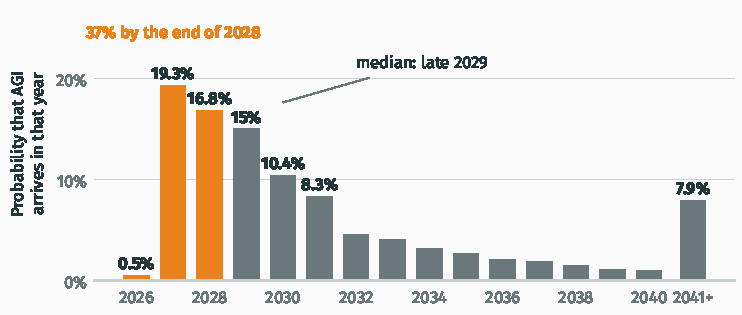
\includegraphics[width=\textwidth]{manifold_agi_year}
\source{manifoldagi2026}
\end{frame}



\begin{frame}{}
\centering
\vfill
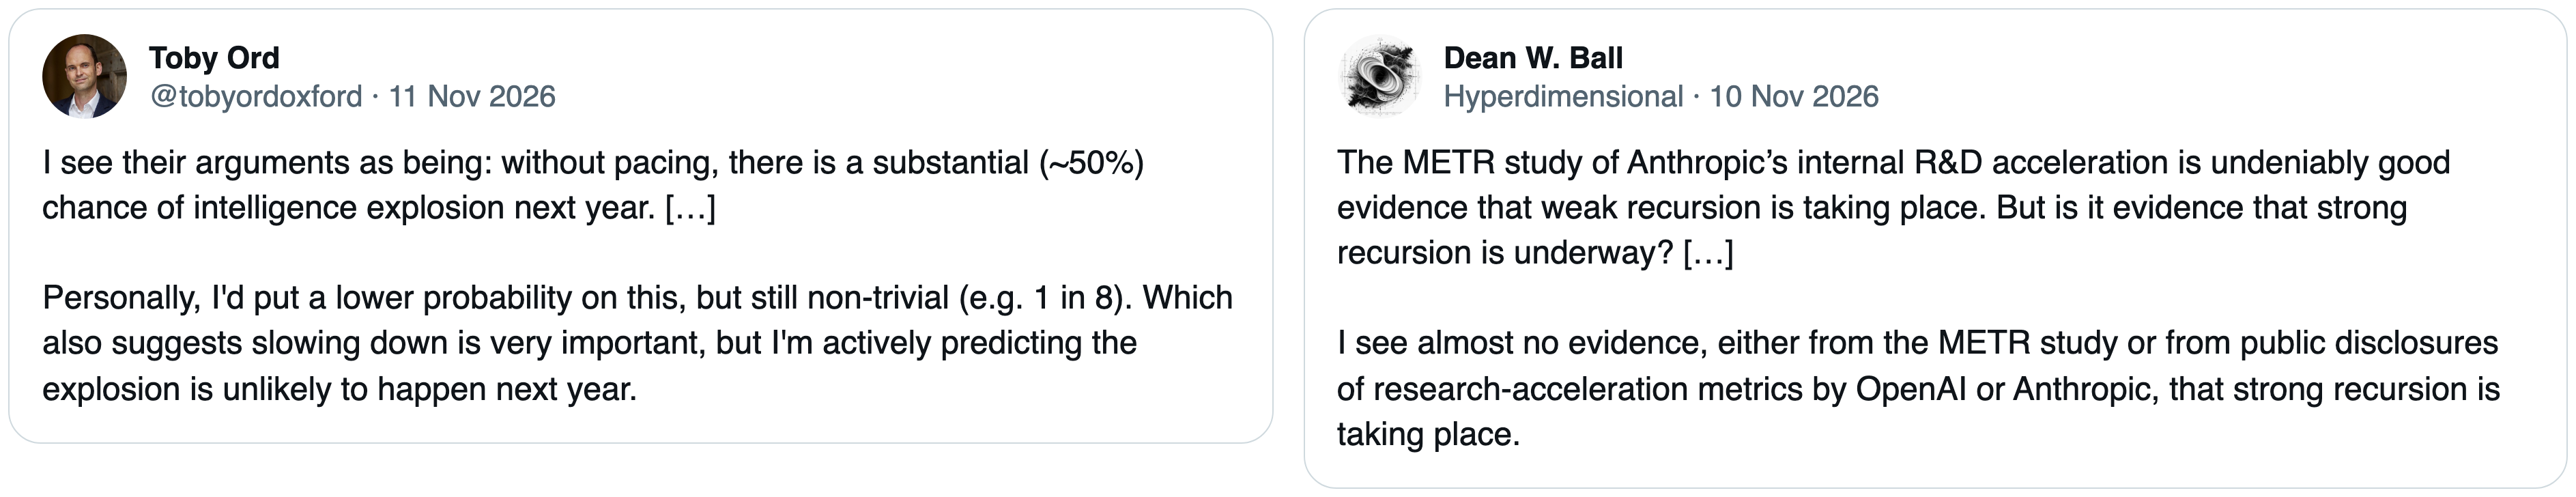
\includegraphics[width=\textwidth,height=0.86\textheight,keepaspectratio]{tweets/skeptics}

\vfill
{\scriptsize\color{gray}10--11 November 2026.
\href{https://x.com/tobyordoxford/status/2120446224478163008}{Ord on X}.
Ball: \href{https://www.hyperdimensional.co/p/iron-makes-iron}{``Iron Makes Iron''}, Hyperdimensional}
\end{frame}

\begin{frame}{Where Is the Mad Scramble?}
\centering
\vfill
{\Large If this were real, would the people in power not be acting like it?}
\vfill
\end{frame}



\section{What Do We Do Now?}
\begin{frame}{If We Believe This, What Changes?}
\begin{columns}[t]
\column{0.31\textwidth}
\centering
{\Huge\faGraduationCap}

\vspace{0.6em}
\textbf{Do not upskill\\for two years}
\column{0.31\textwidth}
\centering
\onslide<2->{
{\Huge\faBolt}

\vspace{0.6em}
\textbf{Do something\\useful soon}
}
\column{0.31\textwidth}
\centering
\onslide<3->{
{\Huge\faRoute}

\vspace{0.6em}
\textbf{Downgrade long\\paths to impact}

\vspace{0.4em}
{\small We will not invent a completely new training paradigm in time}
}
\end{columns}
\end{frame}

\begin{frame}{Three Paths to a Pause Within 6--12 Months}
\vfill
\begin{columns}[t]
\column{0.31\textwidth}
\centering
{\Huge\faFlask}

\vspace{0.6em}
\textbf{Lab advocacy}
\column{0.31\textwidth}
\centering
\onslide<2->{
{\Huge\faGavel}

\vspace{0.6em}
\textbf{California (and Texas)\\state action}
}
\column{0.31\textwidth}
\centering
\onslide<3->{
{\Huge\faLandmark}

\vspace{0.6em}
\textbf{US federal lobbying}
}
\end{columns}
\source{jurkovic2026}
\end{frame}

\begin{frame}{Technical Work That Seems Most Valuable}
\vfill
\begin{columns}[t]
\column{0.31\textwidth}
\centering
{\Huge\faSearch}

\vspace{0.6em}
\textbf{Establishing\\evidence of risk}
\column{0.31\textwidth}
\centering
\onslide<2->{
{\Huge\faBalanceScale}

\vspace{0.6em}
\textbf{Laying the technical foundations for a pause}
}
\column{0.31\textwidth}
\centering
\onslide<3->{
{\Huge\faRobot}

\vspace{0.6em}
\textbf{Aligning and controlling\\the early automated\\researchers}

\vspace{0.4em}
{\small The backup plan, in case a pause does not happen}
}
\end{columns}
\source{jurkovic2026}
\end{frame}

\begin{frame}{For Us Here}
\vfill
\begin{columns}[t]
\column{0.31\textwidth}
\centering
{\Huge\faBrain}

\vspace{0.6em}
\textbf{Make up your own mind}

\vspace{0.4em}
{\small Probably the most important question right now}
\column{0.31\textwidth}
\centering
\onslide<2->{
{\Huge\faComments}

\vspace{0.6em}
\textbf{Talk about it,\\keep your eyes open}

\vspace{0.4em}
{\small And do not throw\\your mind away}
}
\column{0.31\textwidth}
\centering
\onslide<3->{
{\Huge\faMugHot}

\vspace{0.6em}
\textbf{Nothing drastic\\right now}

\vspace{0.4em}
{\small Let the situation sit with you, and keep an eye on it}
}
\end{columns}
\vfill
{\raggedright\scriptsize\color{gray}TsviBT (2023), \textit{Please don't throw your mind away}, LessWrong.\par}
\end{frame}


\begin{frame}[allowframebreaks]{References}
\printbibliography[heading=none]
\end{frame}

\end{document}
